%
% skript.tex -- Skript ueber Klimawandel
%
% (c) 2017 Prof. Dr. Andreas Mueller, HSR
%
\documentclass{book}
\usepackage{etex}
\usepackage{geometry}
\geometry{papersize={170mm,240mm},total={140mm,200mm},top=21mm,bindingoffset=10mm}
\usepackage[english,ngerman]{babel}
\usepackage[utf8]{inputenc}
\usepackage[T1]{fontenc}
\usepackage{cancel}
\usepackage{times}
\usepackage{amsmath,amscd}
\usepackage{amssymb}
\usepackage{amsfonts}
\usepackage{amsthm}
\usepackage[nolist]{acronym}
\usepackage{graphicx}
\usepackage{fancyhdr}
\usepackage{textcomp}
\usepackage[all]{xy}
\usepackage{txfonts}
\usepackage{alltt} 
\usepackage{verbatim}
\usepackage{paralist}
\usepackage{makeidx}
\usepackage{array}
%\usepackage[colorlinks=true]{hyperref}
\usepackage{hyperref}
\usepackage{tikz}
\usepackage{pgfplots}
\usepackage{pgfplotstable}
\usepackage{pdftexcmds}
%\usepackage{pgfmath}
\usepackage{placeins}
\usepackage{subfigure}
\usepackage[autostyle=false,english=american]{csquotes}
\usepackage{float}
\usepackage{enumitem}
\usepackage{wasysym}
\usepackage{environ}
\usepackage{pifont}
\usepackage{feynmp}
\usepackage{appendix}
\usetikzlibrary{calc,intersections,through,backgrounds,graphs,positioning,shapes,arrows,fit}
\usetikzlibrary{patterns,decorations.pathreplacing}
\usetikzlibrary{decorations.pathreplacing}
\usetikzlibrary{external}
\usetikzlibrary{datavisualization}
\usepackage[europeanvoltages,
            europeancurrents,
            europeanresistors,   % rectangular shape
            americaninductors,   % "4-bumbs" shape
            europeanports,       % rectangular logic ports
            siunitx,             % #1<#2>
            emptydiodes,
            noarrowmos,
            smartlabels]         % lables are rotated in a smart way
           {circuitikz}          %
\usepackage{siunitx}
\usepackage{tabularx}
\usetikzlibrary{arrows}

\usepackage{algpseudocode}
\usepackage{algorithm}
\usepackage{gensymb}
\usepackage{mathtools}

% Matlab
\usepackage{listings}
\usepackage{color} %red, green, blue, yellow, cyan, magenta, black, white
\definecolor{mygreen}{RGB}{28,172,0} % color values Red, Green, Blue
\definecolor{mylilas}{RGB}{170,55,241}

\lstset{language=Matlab,%
    %basicstyle=\color{red},
    breaklines=true,%
    morekeywords={matlab2tikz},
    keywordstyle=\color{blue},%
    morekeywords=[2]{1}, keywordstyle=[2]{\color{black}},
    identifierstyle=\color{black},%
    stringstyle=\color{mylilas},
    commentstyle=\color{mygreen},%
    showstringspaces=false,%without this there will be a symbol in the places where there is a space
    numbers=left,%
    %numberstyle={\tiny \color{black}},% size of the numbers
    numbersep=9pt, % this defines how far the numbers are from the text
    emph=[1]{break},emphstyle=[1]\color{red}, %some words to emphasise
    %emph=[2]{word1,word2}, emphstyle=[2]{style},    
}
\lstdefinestyle{Matlab}{
  numbers=left,
  belowcaptionskip=1\baselineskip,
  breaklines=true,
  frame=L,
  xleftmargin=\parindent,
  language=Matlab,
  showstringspaces=false,
  basicstyle=\footnotesize\ttfamily,
  keywordstyle=\bfseries\color{green!40!black},
  commentstyle=\itshape\color{purple!40!black},
  identifierstyle=\color{blue},
  stringstyle=\color{orange},
  numberstyle=\ttfamily\tiny
}
\lstdefinelanguage{Matlab}{
  keywords={function,global,size,zeros,switch,case,otherwise,end,sin,cos,cot,floor,ode45,hold,polarplot},
  sensitive=true
}
\lstdefinelanguage{Maxima}{
  keywords={addrow,addcol,zeromatrix,ident,augcoefmatrix,ratsubst,sum,diff,ev,tex,%
    with_stdout,nouns,express,depends,load,length,submatrix,div,grad,curl,matrix,%
    invert,lambda,facsum,expand,false,then,if,else,subst,batchload,%
    rootscontract,solve,part,assume,sqrt,integrate,abs,inf,exp,sin,cos,sinh,cosh,taylor,ratsimp},
  sensitive=true,
  comment=[n][\itshape]{/*}{*/}
}
\lstdefinestyle{Maxima}{
  numbers=left,
  belowcaptionskip=1\baselineskip,
  breaklines=true,
  frame=L,
  xleftmargin=\parindent,
  language=Maxima,
  showstringspaces=false,
  basicstyle=\footnotesize\ttfamily,
  keywordstyle=\bfseries\color{green!40!black},
  commentstyle=\itshape\color{purple!40!black},
  identifierstyle=\color{blue},
  stringstyle=\color{orange},
  numberstyle=\ttfamily\tiny
}
\lstset{language=Octave,%
    %basicstyle=\color{red},
    breaklines=true,%
    morekeywords={function,global,size,zeros,switch,case,otherwise,end,sin,cos,cot,floor,ode45,hold,polarplot,endfunction,size,endswitch,cat,printf,for,endfor,if,return,endif,abs,while,endwhile},
    keywordstyle=\color{blue},%
    morekeywords=[2]{1}, keywordstyle=[2]{\color{black}},
    identifierstyle=\color{black},%
    stringstyle=\color{mylilas},
    commentstyle=\color{mygreen},%
    showstringspaces=false,%without this there will be a symbol in the places where there is a space
    numbers=left,%
    %numberstyle={\tiny \color{black}},% size of the numbers
    numbersep=9pt, % this defines how far the numbers are from the text
    emph=[1]{break},emphstyle=[1]\color{red}, %some words to emphasise
    %emph=[2]{word1,word2}, emphstyle=[2]{style},    
}
\lstdefinestyle{Octave}{
  numbers=left,
  belowcaptionskip=1\baselineskip,
  breaklines=true,
  frame=L,
  xleftmargin=\parindent,
  language=Octave,
  showstringspaces=false,
  basicstyle=\footnotesize\ttfamily,
  keywordstyle=\bfseries\color{green!40!black},
  commentstyle=\itshape\color{purple!40!black},
  identifierstyle=\color{blue},
  stringstyle=\color{orange},
  numberstyle=\ttfamily\tiny
}
\lstdefinestyle{C}{
  numbers=left,
  belowcaptionskip=1\baselineskip,
  breaklines=true,
  frame=L,
  xleftmargin=\parindent,
  language=C,
  showstringspaces=false,
  basicstyle=\footnotesize\ttfamily,
  keywordstyle=\bfseries\color{green!40!black},
  commentstyle=\itshape\color{purple!40!black},
  identifierstyle=\color{blue},
  stringstyle=\color{orange},
  numberstyle=\ttfamily\tiny
}
\usepackage{caption}
\usepackage[mode=buildnew]{standalone}
\usepackage[backend=bibtex]{biblatex}
% workaround for biblatex bug
\makeatletter
\def\blx@maxline{77}
\makeatother
\addbibresource{references.bib}
% Bibresources für jeden einzelnen Artikel
%\addbibresource{adaptiv/main.bib}
%\addbibresource{cluster/main.bib}
%\addbibresource{cmb/main.bib}
%\addbibresource{gps/main.bib}
%\addbibresource{klima/main.bib}
%\addbibresource{kugel/main.bib}
%\addbibresource{minimal/main.bib}
%\addbibresource{zeitreisen/main.bib}
\AtEndDocument{\clearpage\ifodd\value{page}\else\null\clearpage\fi}
\makeindex
%\pgfplotsset{compat=1.12}
\setlength{\headheight}{15pt} % fix headheight warning
\DeclareGraphicsRule{*}{mps}{*}{}
\begin{document}
\pagestyle{fancy}
\frontmatter
\newcommand\HRule{\noindent\rule{\linewidth}{1.5pt}}
\begin{titlepage}
\vspace*{\stretch{1}}
\HRule
\vspace*{5pt}
\begin{flushright}
{
\LARGE
Mathematisches Seminar\\
\vspace*{20pt}
\Huge
Klimawandel%
}
\vspace*{5pt}
\end{flushright}
\HRule
\begin{flushright}
\vspace{60pt}
\Large
Leitung: Andreas M"uller\\
\vspace{40pt}
\Large
Hansruedi~Patzen,
Melina~Staub,
Martin~Stypinski,
\end{flushright}
\vspace*{\stretch{2}}
\begin{center}
Hochschule f"ur Technik, Rapperswil, 2017
\end{center}
\end{titlepage}
\hypersetup{
    linktoc=all,
    linkcolor=blue
}
\newcounter{beispiel}
\newenvironment{beispiele}{
\bgroup\smallskip\parindent0pt\bf Beispiele\egroup

\begin{list}{\arabic{beispiel}.}
  {\usecounter{beispiel}
  \setlength{\labelsep}{5mm}
  \setlength{\rightmargin}{0pt}
}}{\end{list}}
\newcounter{uebungsaufgabezaehler}
% environment fuer uebungsaufgaben
\newenvironment{uebungsaufgaben}{
\begin{list}{\arabic{uebungsaufgabezaehler}.}
  {\usecounter{uebungsaufgabezaehler}
  \setlength{\labelwidth}{2cm}
  \setlength{\leftmargin}{0pt}
  \setlength{\labelsep}{5mm}
  \setlength{\rightmargin}{0pt}
  \setlength{\itemindent}{0pt}
}}{\end{list}\vfill\pagebreak}
\newenvironment{teilaufgaben}{
\begin{enumerate}
\renewcommand{\labelenumi}{\alph{enumi})}
}{\end{enumerate}}
% Aufgabe
\newcounter{problemcounter}[chapter]
\def\aufgabenpath{chapters/uebungsaufgaben/}
\def\ainput#1{\input\aufgabenpath/#1}
\def\verbatimainput#1{\expandafter\verbatiminput{\aufgabenpath/#1}}
\def\aufgabetoplevel#1{%
\expandafter\def\expandafter\inputpath{#1}%
\let\aufgabepath=\inputpath
}
\def\includeagraphics[#1]#2{\expandafter\includegraphics[#1]{\aufgabepath#2}}
% \aufgabe
\newcommand{\uebungsaufgabe}[1]{%
\refstepcounter{problemcounter}%
\label{#1}%
\bigskip{\parindent0pt\strut}\hbox{\bf\arabic{problemcounter}. }%
\expandafter\def\csname aufgabenpath\endcsname{\inputpath/}%
\expandafter\input{chapters/uebungsaufgaben/#1.tex}
}
\renewcommand\theproblemcounter{\thechapter.\arabic{problemcounter}}

% Loesung
\def\swallow#1{
%nothing
}
\NewEnviron{loesung}[1][L"osung]{%
\begin{proof}[#1]%
\renewcommand{\qedsymbol}{$\bigcirc$}
\BODY
\end{proof}
}
\NewEnviron{bewertung}{%
\begin{proof}[Bewertung]%
\renewcommand{\qedsymbol}{}
\BODY
\end{proof}
}
\NewEnviron{diskussion}{%
\begin{proof}[Diskussion]%
\renewcommand{\qedsymbol}{}
\BODY
\end{proof}
}
\NewEnviron{hinweis}{%
\begin{proof}[Hinweis]%
\renewcommand{\qedsymbol}{}
\BODY
\end{proof}
}
\def\keineloesungen{%
\RenewEnviron{loesung}{\relax}
\RenewEnviron{bewertung}{\relax}
\RenewEnviron{diskussion}{\relax}
}
\newenvironment{beispiel}{%
\begin{proof}[Beispiel]%
\renewcommand{\qedsymbol}{$\bigcirc$}
}{\end{proof}}

\allowdisplaybreaks

\lhead{Inhaltsverzeichnis}
\rhead{}
\tableofcontents
\newtheorem{satz}{Satz}[chapter]
\newtheorem{hilfssatz}[satz]{Hilfssatz}
\newtheorem{definition}[satz]{Definition}
\newtheorem{annahme}[satz]{Annahme}
\newtheorem{problem}[satz]{Problem}
\newtheorem*{problem*}{Problem}
\renewcommand{\floatpagefraction}{0.7}
\mainmatter
%
% vorwort.tex -- Vorwort zum Buch zum Seminar
%
% (c) 2017 Prof Dr Andreas Mueller, Hochschule Rapperswil
%
\chapter*{Vorwort}
\lhead{Vorwort}
\rhead{}
Dieses Buch entstand im Rahmen des Mathematischen Seminars
im Frühjahrssemester 2017 an der Hochschule für Technik Rapperswil.
Die Teilnehmer, Studierende der Abteilungen für Elektrotechnik,
Informatik und Bauingenieurwesen der
HSR, erarbeiteten nach einer Einführung in das Themengebiet jeweils
einzelne Aspekte des Gebietes in Form einer Seminararbeit, über
deren Resultate sie auch in einem Vortrag informierten. 

Im Frühjahr 2018 war das Thema des Seminars der Klimawandel.

Im zweiten Teil dieses Skripts kommen dann die Teilnehmer selbst zu Wort.
Ihre Arbeiten wurden jeweils als einzelne
Kapitel mit meist nur typographischen Änderungen übernommen.
Diese weiterführenden Kapitel sind sehr verschiedenartig.
Eine Übersicht und Einführung findet sich in der Einleitung
zum zweiten Teil auf Seite~\pageref{skript:uebersicht}.

In einigen Arbeiten wurde auch Code zur Demonstration der 
besprochenen Methoden und Resultate geschrieben, soweit
möglich und sinnvoll wurde dieser Code im Github-Repository
dieses Kurses%
\footnote{\url{https://github.com/AndreasFMueller/SeminarKlima.git}}
abgelegt.

Im genannten Repository findet sich auch der Source-Code dieses
Skriptes, es wird hier unter einer Creative Commons Lizenz
zur Verfügung gestellt.
Auf der beiliegenden DVD befinden sich die Testdaten und Programme
zu zwei der simulationsintensiveren Artikel im zweiten Teil.



\part{Grundlagen}
%\keineloesungen
\begin{refsection}
%\section{THC, Was ist das?}
\rhead{THC, Was ist das?}

Die "THC", ausgeschrieben thermohaline Zirkulation. Ist eine Weltumspannende Meeresströmung welche in verschiedene Abschnitte aufgeteilt werden kann.
Diese Strömungen sorgen für eine Durchmischung der verschiedenen Ozeane. So erzeugen sie einen Wärme- und Nährstoffaustausch in den verschiedenen Weltregionen. 
Die Auswirkung dieses Energieaustausches sind spürbar, so heizt zum Beispiel der Golfstrom, welcher Auch zu diesen Strömungen gehört Nordeuropa um mehrere Grad auf.
Doch wie entsteht diese Strömung?
Hier spielen viele Einflüsse eine Rolle. Die Verteilung der Kontinente, die Corioliskraft, die Wasserdichte und auch Wetter und Winde. 
Im Rahmen dieser Arbeit werde ich nur auf die Wasserdichte als Einfluss eingehen. Sie ist gut zu simulieren und ist durch die einfache Veränderbarkeit auch am Spannendsten.
die Verteilung der Kontinente und auch die Corioliskraft sind durch ihre kaum vorhandene Änderung als Konstanten zu betrachten. Das Letzte was noch bleibt, sind Wind und Wetter. 
Diese Einflüsse sind praktisch nicht vorherzusagen und auch ihr Einfluss variiert stark. Aus diesem Grund werden auch diese nicht Simuliert. 
Zusätzlich würde das Einbeziehen dieser grössen die Komplexität der Simulation Stark erhöhen.

\subsection{Dichte}
\rhead{Dichte}

Die Thermohaline Zirkulaton wird hauptsächlich durch Dichteunterschiede im Wasser hervorgerufen.
Dichtes Wasser sinkt ab und weniger dichtes Wasser steigt bekanntlich auf. Die Hauptsächlichen Einflussfaktoren der Wasserdichte sind:

\begin{itemize}
	\item Salzgehalt
	\item Temperatur
\end{itemize}

Durch einen hohen Salzgehalt wird das Wasser dichter. Die Temperatur hat den inversen Einfluss. Je wärmer das Wasser wird, desto weniger dicht ist es. 
Hier zwei Grafiken zur Veranschaulichung:
\begin{figure}
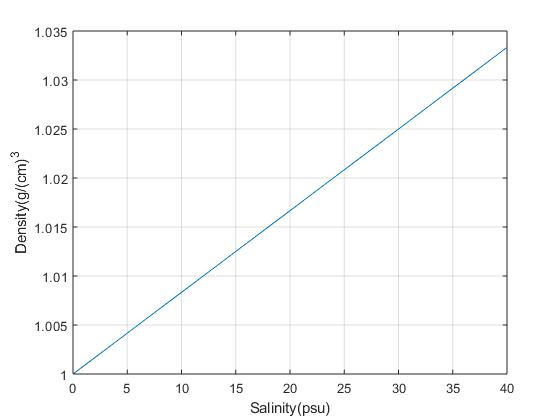
\includegraphics{code/graphs/graph_salinity.jpg}
\caption{Dichteveränderung abhängig vom Salzgehalt}
\end{figure}

\begin{figure}
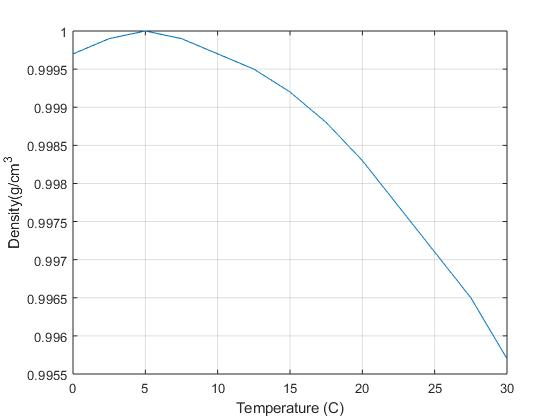
\includegraphics{code/graphs/graph_temp.jpg}
\caption{Dichteveränderung abhängig von der Temperatur}
\end{figure}

Diese Einflüsse Lassen sich in einer Gleichung zusammenfassen, welche im Hauptteil des Buches im Kapitel \ref{Salinität und Dichte} schon Besprochen wurde.

\begin{equation}
\varrho
=
\varrho_0(1-\alpha(T-T_0)+\beta(S-S_0))
\label{skript:salinity-linear}
\end{equation} 

Mittels dieser Gleichung lässt sich nun ein Simulation erstellen, mit welcher sich solche Strömungen simulieren lassen.

\subsection{Golfstrom}
\rhead{Golfstrom}

Im Rahmen dieser Arbeit habe ich versucht den Golfstrom, welcher Europa direkt beeinflusst, zu Simulieren.
Als fokussieren ich hier nur auf einen kleinen Teil der Globalen Thermohalinen Zirkulation.


\begin{figure}
	\includegraphics[]{bilder/deep_ocean_currents.jpg}
\end{figure}

Die Frage ist nun, was passiert mit dem Golfstrom, wenn Klimaerwärmung und Umweltverschmutzung weiter ansteigen?

\subsubsection{Funktionsweise}

Doch zuerst dazu, wie der Golfstrom funktioniert.
Der Golfstrom entspringt im Golf von Mexiko. Von dort aus wird das Warme Wasser von Winden und der Erdrotation nach Norden getrieben.
Auf diesem Weg kühlt das Wasser langsam ab, und wird durch die fortlaufende Verdunstung von Wasser immer salziger. Da der Einfluss der Salinität grösser ist als der der Temperatur, beginnt das Wasser im Norden, durch die nun Hohe Dichte abzusinken. Wenn das Wasser dann abgesunken ist, treibt es dem Grund des Meeres entlang bis nach Afrika, was den Kreislauf schliesst.
Wo hat der Klimawandel nun seinen Einfluss?
Um diese Frage zu beantworten, müssen wir weiter zurückschauen, genauer gesagt zum Kap der guten Hoffnungen. Denn eigentlich beginnt die Strömung schon dort. 
Dort Stellt sich die Frage, in welcher Richtung der Indische Ozean und der Atlantik ihr Salz austauschen. 
Denn eine Veränderung der Salzbilanz könnte im Norden, also vor der Küste Grönlands für eine Störung des Absinkens sorgen, und so den Strom zum erliegen bringen. 
Eine Störung der Salzzufuhr könnte also den Golfstrom zum erliegen bringen.
Hier gehen die Meinungen der Forscher jedoch auseinander. Salzmessungen im offenen Meer sind sehr schwierig. 
Im Moment zeigen diese jedoch, dass der Golfstrom weiter Salz in den Atlantik importiert und sich so selber am leben erhält.

Weiter kommt da noch die Erhöhung des CO2-Gehaltes in der Luft und die somit einhergehende Klimaerwärmung. sie hat zwei direkte Auswirkungen auf den Golfstrom:

\begin{itemize}
	\item Durch die Erhöhung der Lufttemperatur kann das Wasser auf dem Weg in den Norden nicht mehr genug abkühlen, um danach abzusinken.
	\item Das Abschmelzen der Polkappen, welches viel Frischwasser freisetzt, kann die Salzkonzentration so weit verringern, dass das Wasser, aufgrund der reduzierten Dichte, nicht mehr absinken kann.
\end{itemize}

Diese Beiden Prozesse, wären alleine in der Lage den Golfstrom zu stören, doch zusammen ist die Wirkung noch viel schlimmer.

Laut einer Studie des Forschers Liu Wei von der Universität Yale vom 04 Jan 2017 könnte dieses Szenario in den nächsten 300 Jahren tatsächlich eintreten. Sie zeigen auf, dass falls sich die Rate seit 1990 verdoppelt, der Golfstrom in den nächsten 300 Jahren versiegen könnte.

\subsubsection{Folgen}

Was passiert, falls der Golfstrom zum erliegen kommt, oder sogar seine Richtung ändert.
Ich denke der Film "The day after tomorrow" von Roman Emmerich ist bekannt. Er zeigt was passieren könnte, falls der Golfstrom zum erliegen kommt. 
Im Film versinkt innert weniger Tage die ganze Welt in einer neuen Eiszeit un alles endet im Chaos. 
Das ist natürlich ein wenig übertrieben Dargestellt, doch die Richtung stimmt. Falls der Golfstrom stoppt, würde trotz Klimaerwärmung Nordeuropa um einige Grad kälter werden.













	
	
	
	
	
	
	
	
	
	
	
	
	
\end
%\input{chapters/kurven.tex}
%\input{chapters/laengenmessung.tex}
%\input{chapters/geodaeten.tex}
%\input{chapters/kruemmung.tex}
%\input{chapters/speziell.tex}
%\input{chapters/gravitation.tex}
%\input{chapters/schwarzschild.tex}
%\input{chapters/robertson.tex}
%\input{chapters/friedmann.tex}
%\input{chapters/multipol.tex}
%%
% kugelfunktionen.tex -- Kugelfunktionen
%
% (c) 2018 Prof Dr Andreas Müller, Hochschule Rapperswil
%
\subsection{Kugelfunktionen}
Die Basisfunktionen im Lorenz-Modell waren aus zwei Gründen besonders
erfolgreich.
\begin{enumerate}
\item
Die Basisfunktionen waren Produkte von Funktionen, die jeweils nur von
einer Koordinate abhängen.
In einem Produkt 
$f(x,y)=X(x)\cdot Y(y)$ 
sind die Ableitungen nach den Koordinaten besonders einfach auszurechnen,
da gilt
\[
\begin{aligned}
\frac{\partial f}{\partial x}(x,y) &= X'(x)\cdot Y(y)
&&\text{und}&
\frac{\partial f}{\partial y}(x,y) &= X(x)\cdot Y'(y).
\end{aligned}
\]
\item
Die Basisfunktionen waren Eigenfunktionen des Laplace-Operators, also
\[
\Delta f = \lambda f.
\]
Da in den Gleichungen der Strömungsdynamik der Laplace-Operator
prominent vorkommt, bedeutet diese Eigenschaft, dass die Wirkung des
Laplace-Operators auf die Basisfunktionen durch Multiplikation mit
dem Eigenwert ersetzt werden kann.
Dadurch werden die Gleichungen sehr vereinfacht und die Ordnung
der Differentialgleichung reduziert sich.
\end{enumerate}
Wenn der Erfolg der speziellen Basiswahl im Lorenz-System für ein
Wetter- oder Klimamodell auf der Kugeloberfläche repliziert werden
soll, dann ist nahe liegend, dass dazu Funktionen mit den gleichen
Eigenschaften in Kugelkoordinaten gefunden werden müssen.

\subsubsection{Separationsansatz}
Die Produkteigenschaft bedeutet, dass die Basisfunktionen in der Form
\[
f(r,\varphi,\vartheta)
=
R(r)\cdot \Phi(\varphi)\cdot \Theta(\vartheta)
\]
gefunden werden müssen.
Das in Abschnitt~\ref{section:pdeloesungen} dargestellte
Separationsverfahren für partielle
Differentialgleichungen~\cite[Chapter 4]{skript:pde}
basiert genau auf dieser Art von Ansatz.

\subsubsection{Eigenwertgleichung}
Die Eigenwerteigenschaft bedeutet, dass die Funktionen Eigenfunktionen
des Laplace-Operators sein müssen, also Lösungen der partiellen
Differentialgleichungen
\[
\Delta f = \lambda f.
\]
Wenden wir den Laplace-Operator in Kugelkoordinaten auf $f$ an, finden
wir
\begin{align*}
\Delta f
&=
\biggl(
\frac{1}{r^2} \frac{\partial}{\partial r}
\biggl(r^2\frac{\partial f}{\partial r}\biggr)
+
\frac1{r^2\sin\vartheta}\frac{\partial}{\partial\vartheta}
\biggl(\sin\vartheta\frac{\partial f}{\partial\vartheta}\biggr)
+
\frac1{r^2\sin^2\vartheta}\frac{\partial^2 f}{\partial\varphi^2}
\biggr)
R(r)\cdot \Phi(\varphi)\cdot \Theta(\vartheta)
\\
&=
\frac1{r^2}\frac{\partial}{\partial r}\bigl(r^2R'(r)\bigr)
\cdot \Theta(\vartheta)\cdot \Phi(\varphi)
+
\frac1{r^2\sin\vartheta}\frac{d}{d\vartheta}
\bigl(\sin\vartheta \Theta'(\vartheta)\bigr)
\cdot R(r)\cdot \Phi(\varphi)
\\
&\qquad
+
\frac1{r^2\sin^2\vartheta}\Phi''(\varphi)
\cdot R(r)\cdot \Theta(\vartheta)
\\
&=
\frac1{r^2}\bigl(2rR'(r)+r^2R''(r)\bigr)
\Theta(\vartheta)\Phi(\varphi)
+
\frac1{r^2\sin\vartheta}
\bigl(\sin\vartheta\Theta'(\vartheta)\bigr)'
\cdot R(r)\cdot\Phi(\varphi)
\\
&\qquad
+
\frac1{r^2\sin^2\vartheta}
\Phi''(\varphi)
\cdot R(r)\cdot \Theta(\vartheta)
\\
&=
\lambda
R(r)\cdot \Theta(\vartheta)\cdot \Phi(\varphi).
\end{align*}

\subsubsection{Separation von $r$}
Um die einzelnen Funktionen zu isolieren, teilen wir durch $f$.
Zwar kann $f$ Nullstellen haben, aber für die meisten Werte der Koordinaten
ist $f$ von Null verschieden, für diese Punkte ist die Division unproblematisch
und ausreichend, um die Faktoren zu bestimmen.
Wir erhalten
\begin{align*}
\frac{2rR'(r)+r^2R''(r)}{r^2R(r)}
+
\frac{
\bigl(\sin\vartheta\Theta'(\vartheta)\bigr)'
}{r^2\sin\vartheta\Theta(\vartheta)}
+
\frac{1}{r^2\sin^2\vartheta}\frac{\Phi''(\varphi)}{\Phi(\varphi)}
&=\lambda
\end{align*}
Um die Variable $r$ allein auf die linke Seite zu bringen, multiplizieren wir
mit $r^2$, subtrahieren $\lambda r^2$ und bringen den zweiten und dritten 
Term auf der linken Seite auf die rechte Seite.
So erhalten wir
\begin{align*}
\frac{r^2R''(r)+2rR'(r)-\lambda r^2R(r)}{R(r)}
&=
-
\frac{
\bigl(\sin\vartheta\,\Theta'(\vartheta)\bigr)'
}{\sin\vartheta\,\Theta(\vartheta)}
-\frac{1}{\sin^2\vartheta}\frac{\Phi''(\varphi)}{\Phi(\varphi)}
\end{align*}
Die linke Seite hängt nur von $r$ ab, die rechte Seite nur von $\vartheta$
und $\varphi$.
Dies ist nur möglich, wenn beide Seiten konstant sind.
Es gibt also ein Zahl $\mu$ derart, dass
\begin{align}
\frac{r^2R''(r)+2rR'(r)-\lambda r^2R(r)}{R(r)}&=\mu,
\\
\frac{\bigl(\sin\vartheta\,\Theta'(\vartheta)\bigr)'}{\sin\vartheta\,\Theta(\vartheta)}
+
\frac{1}{\sin^2\vartheta}\frac{\Phi''(\varphi)}{\Phi(\varphi)}
&=
-\mu.
\label{skript:kugel:thetaphi}
\end{align}
Die erste Gleichung kann man vereinfachen zu
\begin{equation}
r^2R''(r)+2rR'(r)-(\lambda r^2-\mu)R(r) = 0,
\end{equation}
eine gewöhnliche lineare Differentialgleichung zweiter Ordnung.
$\mu$ kann nicht beliebig gewählt werden, der Wert muss so sein,
dass \eqref{skript:kugel:thetaphi} gelöst werden kann.

Doch auch $\lambda$ ist nicht beliebig, sein Wert muss so gewählt
werden, dass eventuelle Randbedingungen für die zugehörigen Funktion
$R(r)$ erfüllt sind.
Da die $r$-Abhängigkeit für die folgende Diskussion nicht wichtig ist,
verfolgen wir diese Frage hier nicht weiter.

\subsubsection{Separation von $\vartheta$ und $\varphi$}
Die Gleichung~\eqref{skript:kugel:thetaphi} enthält nur noch die
Variablen $\vartheta$ und $\varphi$. 
Wir versuchen den gleichen Trick erneut: indem wir mit $\sin^2\vartheta$
multiplizieren, den Term mit $\mu$ auf die linke Seite bringen und
den zweiten Term auf die rechte Seite bringen, erhalten wir
\[
\sin\vartheta
\frac{1}{\Theta(\vartheta)}
\frac{d}{d\vartheta}\bigl(\sin\vartheta\,\Theta'(\vartheta)\bigr)
+
\mu\sin^2\vartheta
=
-\frac{\Phi''(\varphi)}{\Phi(\varphi)}.
\]
Erneut haben wir eine Gleichung, deren linke Seite nur von $\vartheta$
und deren rechte Seite nur von $\varphi$ abhängt.
Also sind wieder beide Seiten konstant, es gibt also eine Konstante
$\nu$ derart, dass $\Theta(\vartheta)$ und $\Phi(\varphi)$ die 
Gleichungen
\begin{align}
\sin\vartheta\frac{d}{d\vartheta}
\biggl(
\sin\vartheta\frac{d}{d\vartheta}\Theta(\vartheta)
\biggr)
&=
(-\mu\sin^2\vartheta+\nu)\Theta(\vartheta)
\label{skript:kugel:thetagl}
\\
-\frac{\Phi''(\varphi)}{\Phi(\varphi)}&=\nu
\label{skript:kugel:phigl}
\end{align}
erfüllen.

\subsubsection{Lösungsfunktionen $\Phi(\varphi)$}
Die zweite Gleichung~\eqref{skript:kugel:phigl} ist gleichbedeutend mit
\begin{equation}
\Phi''(\varphi)=-\nu\Phi(\varphi),
\label{skript:kugel:philsg}
\end{equation}
wobei $\Phi(\varphi)$ eine $2\pi$-periodische Funktion ist.
Die Lösungen der Gleichung~\eqref{skript:kugel:philsg}
sind $\cos\sqrt{\nu}\varphi$ und $\sin\sqrt{\nu}\varphi$,
aber die Periodizität verlangt, dass $\sqrt{\nu}$ eine ganze Zahl ist.
Es muss also gelten $\nu=k^2$ mit $k\in \mathbb N$.

\subsubsection{Lösungsfunktionen $\Theta(\vartheta)$}
Im vorangegangen Absatz wurde gezeigt, dass $\nu=k^2$ ist, was die
Gleichung~\eqref{skript:kugel:thetagl} zu
\begin{equation}
\sin\vartheta\frac{d}{d\vartheta}\sin\vartheta\frac{d}{d\vartheta}\Theta(\vartheta)
=
\biggl(\sin\vartheta\frac{d}{d\vartheta}\biggr)^2 \Theta(\vartheta)
=
(-\mu\sin^2\vartheta+k^2)\Theta(\vartheta)
\label{skript:kugel:legendredgl0}
\end{equation}
In dieser Form ist die Differentialgleichung nicht so leicht zu
erkennen.
Schreibt man aber $z=\sin\vartheta$, dann wird die Ableitung einer
Funktion $P(z)=\Theta(\vartheta)$
\begin{align*}
\frac{d}{d\vartheta}\Theta(\vartheta)
=
\frac{d}{d\vartheta}P(\cos\vartheta)
=
-P'(\cos\vartheta) \sin\vartheta
&=
-\sqrt{1-\cos^2\vartheta}P'(\cos\vartheta)
\\
&=
-\sqrt{1-z^2}P'(z)
=
-\sqrt{1-z^2}\frac{d}{dz}P(z).
\end{align*}
Ableitungen nach $\vartheta$ sind also zu ersetzen durch Ableitungen
nach $z$ gefolgt von Multiplikation mit $-\sqrt{1-z^2}$.
In der Differentialgleichung~\eqref{skript:kugel:legendredgl0}
wird die Ableitung nach $\vartheta$ jeweils auch noch mit $\sin\vartheta=\sqrt{1-z^2}$
multipliziert.
Der Operator
\begin{equation}
\sin\vartheta\frac{d}{d\vartheta}
\qquad
\text{bekommt daher die Form}
\qquad
-(1-z^2)\frac{d}{dz}.
\label{skript:kugel:zoperator}
\end{equation}
Das Vorzeichen ist nicht wichtig, da der Operator in der Differentialgleichung
\eqref{skript:kugel:legendredgl0} nur im Quadrat vorkommt.

Wir setzen jetzt die Form \eqref{skript:kugel:zoperator}
des Differentialoperators in die Differentialgleichung
\eqref{skript:kugel:legendredgl0} ein
und erhalten 
\begin{align}
(1-z^2)\frac{d}{dz}\bigl((1-z^2)P'(z)\bigr)
&=
(-\mu(1-z^2)+m^2)P(z)
\notag
\\
\Rightarrow\qquad
(1-z^2)P''(z) -2z P'(z)
+
\mu P(z)
-\frac{m^2}{1-z^2}P(z)
&=
0.
\label{skript:kugel:legendredgl}
\end{align}
Für $m=0$ ist
\eqref{skript:kugel:legendredgl}
die sogenannte Legendresche Differentialgleichung.
\index{Differentialgleichung!Legendresche}
\index{Legendresche Differentialgleichung}
Sie hat Lösungen für $\mu=l(l+1)$ mit $l\in\mathbb N$.
Für $m>0$ ist
\eqref{skript:kugel:legendredgl}
die assozierte Legendre-Differentialgleichung.
Für beide Gleichung lassen sich Lösungen angeben, es sind die
sogenannten Legendre-Polynome $P_l(z)$ im Fall $m=0$ und die zugeordneten
Legendre-Polynome $P_l^m(z)$ für beliebiges $m$.

\subsubsection{Kugelflächenfunktionen}
Mit den gefundenen Lösungen für $\Phi(\varphi)$ und $\Theta(\vartheta)$
finden wir jetzt die allgemeinen Lösungen 
der Differentialgleichung \eqref{skript:kugel:thetaphi}.
Es sind die Funktionen
\[
Y_l^m(\vartheta,\varphi)
=
N_{lm}
P_l^m(\cos\vartheta) e^{im\varphi}
\]
mit einem geeigneten Normierungsfaktor $N_{lm}$.
Diese Funktionen haben genau die Eigenschaften, die wir in der Einleitung
dieses Abschnitts als Voraussetzungen für eine geeignete Basis
gefordert haben.




%\input{chapters/cmb.tex}
%\input{kapitel.tex}
\begin{appendices}
%\input{chapters/konstanten.tex}
%\input{chapters/komplexezahlen.tex}
\end{appendices}
\vfill
\pagebreak
\ifodd\value{page}\else\null\clearpage\fi
\lhead{Literatur}
\rhead{}
\printbibliography[heading=subbibliography]
\label{skript:literatur}
\end{refsection}

\part{Anwendungen und Weiterf"uhrende Themen}
\lhead{Anwendungen}
%
% uebersicht.tex -- Uebersicht ueber die Seminar-Arbeiten
%
% (c) 2018 Prof Dr Andreas Mueller, Hochschule Rapperswil
%
\chapter*{"Ubersicht}
\lhead{"Ubersicht}
\rhead{}
\label{skript:uebersicht}
Im zweiten Teil kommen die Teilnehmer des Seminars selbst zu Wort.
Die im ersten Teil dargelegten mathematischen Methoden und
grundlegenden Modelle werden dabei verfeinert, verallgemeinert
und auch numerisch überprüft.
Die Beispiele zeigen auch, dass umfassende Klimamodell erwartungsgemäss
schnell sehr komplex werden können.
Sie zeigen aber auch, dass es möglich ist, wesentliche Aspekte
des Klimas aus einfachen Überlegungen und mit übersichtlichen
mathematischen Modellen zu erfassen und zu verstehen.

{\em Matthias Baumann} und {\em Oliver Dias} zeigen zusätzliche
Informationen zum Lorenz-System, insbesondere zum Lorenz-Attraktor.
{\em Hansruedi Patzen} verallgemeinert das Vorgehen, mit dem das
Lorenz-System gewonnen wurde, im Sinne des Separationsverfahrens
für partielle Differentialgleichungen weiter, und gewinnt eine
Reihe von höherdimensionalen Lorenz-Systemen und untersucht weiter,
ob das beim dreidimensionalen System gefundene chaotische Verhalten 
auch in den höherdimensionalen Versionen zu finden ist.
Diese Untersuchungen zeigen, dass das Verhalten wahrscheinlich
nicht nur ein Artefakt der Reduktion auf drei Dimensionen ist, sondern
eine inhärente Eigenschaft des Lorenz-Systems.

Die exakte Lösung von Klimamodellen ist oft sehr schwierig, oft sind
Parameter oder Abhängigkeiten nicht bekannt.
Ein alternativer Ansatz ist daher, die zeitliche Entwicklung
im Sinne von machine learning zu lernen.
{\em Martin Stypinski} untersucht diesen Ansatz an zwei Beispielen,
der Wärmeleitungsgleichung und der nichtlinearen Gleichung von Burgers.
Die Beispiele zeigen vor allem auch, wie mathematisches Wissen über das
Modell hilft, die neuronalen Netzwerke zweckmässig zu entwerfen.

Die im Text entwickelten Modelle sind meist noch rudimentär, eine
reihe von Arbeiten haben sich daher mit Erweiterungen und Verfeinerungen
befasst.
{\em Jonas Gründler} hat das 2-Box Modell der thermohalinen Zirkulation
auf 3 Boxen verallgemeinert.
{\em Silvio Marti} studiert den Einfluss von Eis auf das Klima.
Die verzögerte Differentialgleichung des El Niño-Systems kann
numerische gelöst werden. {\em Raphael Unterer} zeigt, wie dies
funktioniert und findet insbesondere auch eine Stabilitätsbedingung
für sein Verfahren.
{\em Nicolas Tobler} hat versucht, die Modelle auf verschiedene
Planeten zu verallgemeinern und damit die Unterschiede der Atmosphären
der Planeten Venus, Erde und Mars zu erklären.
Die Einflüsse anderer Planeten zeigen sich zum Beispiel in der
Neigung der Erdachse gegen die Erdbahnebene.
Wie {\em Sebastian Lenhard} vorführt, können auch kleine Änderungen
der Neigung das Klima dramatisch verändern.
%Schliesslich gibt es auch eine Kopplung zwischen Klima und
%Vegetation, die {\em Matthias Dunkel} modelliert hat.

Die letzten zwei Kapitel befassen sich mit der Aufarbeitung der
Daten, auf grund derer wir zum Schluss kommen, dass 
der Klimawandel real ist.
Für Wetter- wie auch für Klimamodelle sind grosse Datenmengen
von Wetter- und Klimamessstationen in die Rechnung zu integrieren.
Der Kalman-Filter ist die Basis vieler moderner Lösungsansätze
für dieses Problem.
Am Beispiel des erweiterten Kalman-Filters für das Lorenz-System
zeigt {\em Michael Müller}, wie es möglich ist, den Systemzustand
selbst eines chaotischen nichtlinearen Systems zu 
Extreme Ereignisse sind in den letzten Jahren häufiger geworden
und werden oft als Indikatoren für die Klimaveränderung angeführt.
Wie man mit statistischen Daten über solche Ereignisse beweisen
kann, dass der Klimawandel tatsächlich stattfindet, zeigt
{\em Melina Staub}.






\def\chapterauthor#1{{\large #1}\bigskip\bigskip}
% Artikel
%%
% main.tex -- Paper zum Thema <thema>
%
% (c) 2018 Hochschule Rapperswil
%
\chapter{Achsneigung und Eiszeiten\label{chapter:thema}}
\lhead{Achseneigung und Eiszeiten}
\begin{refsection}
\chapterauthor{Sebastian Lenhard}

\section{Abschnitt}
\rhead{Abschnitt}

\section{Schlussfolgerung}
\rhead{Schlussfolgerung}

\printbibliography[heading=subbibliography]
\end{refsection}

%%
% main.tex -- Paper zum Thema <thema>
%
% (c) 2018 Hochschule Rapperswil
%
\chapter{Achsneigung und Eiszeiten\label{chapter:thema}}
\lhead{Achseneigung und Eiszeiten}
\begin{refsection}
\chapterauthor{Sebastian Lenhard}

\section{Abschnitt}
\rhead{Abschnitt}

\section{Schlussfolgerung}
\rhead{Schlussfolgerung}

\printbibliography[heading=subbibliography]
\end{refsection}

%%
% main.tex -- Paper zum Thema <thema>
%
% (c) 2018 Hochschule Rapperswil
%
\chapter{Achsneigung und Eiszeiten\label{chapter:thema}}
\lhead{Achseneigung und Eiszeiten}
\begin{refsection}
\chapterauthor{Sebastian Lenhard}

\section{Abschnitt}
\rhead{Abschnitt}

\section{Schlussfolgerung}
\rhead{Schlussfolgerung}

\printbibliography[heading=subbibliography]
\end{refsection}

%%
% main.tex -- Paper zum Thema <thema>
%
% (c) 2018 Hochschule Rapperswil
%
\chapter{Achsneigung und Eiszeiten\label{chapter:thema}}
\lhead{Achseneigung und Eiszeiten}
\begin{refsection}
\chapterauthor{Sebastian Lenhard}

\section{Abschnitt}
\rhead{Abschnitt}

\section{Schlussfolgerung}
\rhead{Schlussfolgerung}

\printbibliography[heading=subbibliography]
\end{refsection}

%%
% main.tex -- Paper zum Thema <thema>
%
% (c) 2018 Hochschule Rapperswil
%
\chapter{Achsneigung und Eiszeiten\label{chapter:thema}}
\lhead{Achseneigung und Eiszeiten}
\begin{refsection}
\chapterauthor{Sebastian Lenhard}

\section{Abschnitt}
\rhead{Abschnitt}

\section{Schlussfolgerung}
\rhead{Schlussfolgerung}

\printbibliography[heading=subbibliography]
\end{refsection}

%%
% main.tex -- Paper zum Thema <thema>
%
% (c) 2018 Hochschule Rapperswil
%
\chapter{Achsneigung und Eiszeiten\label{chapter:thema}}
\lhead{Achseneigung und Eiszeiten}
\begin{refsection}
\chapterauthor{Sebastian Lenhard}

\section{Abschnitt}
\rhead{Abschnitt}

\section{Schlussfolgerung}
\rhead{Schlussfolgerung}

\printbibliography[heading=subbibliography]
\end{refsection}

%%
% main.tex -- Paper zum Thema <thema>
%
% (c) 2018 Hochschule Rapperswil
%
\chapter{Achsneigung und Eiszeiten\label{chapter:thema}}
\lhead{Achseneigung und Eiszeiten}
\begin{refsection}
\chapterauthor{Sebastian Lenhard}

\section{Abschnitt}
\rhead{Abschnitt}

\section{Schlussfolgerung}
\rhead{Schlussfolgerung}

\printbibliography[heading=subbibliography]
\end{refsection}

%%
% main.tex -- Paper zum Thema <thema>
%
% (c) 2018 Hochschule Rapperswil
%
\chapter{Achsneigung und Eiszeiten\label{chapter:thema}}
\lhead{Achseneigung und Eiszeiten}
\begin{refsection}
\chapterauthor{Sebastian Lenhard}

\section{Abschnitt}
\rhead{Abschnitt}

\section{Schlussfolgerung}
\rhead{Schlussfolgerung}

\printbibliography[heading=subbibliography]
\end{refsection}

\vfill
\pagebreak
\ifodd\value{page}\else\null\clearpage\fi
\lhead{Index}
\rhead{}
\addcontentsline{toc}{chapter}{\indexname}
%
% skript.tex -- Skript ueber Klimawandel
%
% (c) 2017 Prof. Dr. Andreas Mueller, HSR
%
\documentclass{book}
\usepackage{etex}
\usepackage{geometry}
\geometry{papersize={170mm,240mm},total={140mm,200mm},top=21mm,bindingoffset=10mm}
\usepackage[english,ngerman]{babel}
\usepackage[utf8]{inputenc}
\usepackage[T1]{fontenc}
\usepackage{cancel}
\usepackage{times}
\usepackage{amsmath,amscd}
\usepackage{amssymb}
\usepackage{amsfonts}
\usepackage{amsthm}
\usepackage{graphicx}
\usepackage{fancyhdr}
\usepackage{textcomp}
\usepackage{txfonts}
%\usepackage{alltt} 
\newcommand\hmmax{0}
\newcommand\bmmax{0}
\usepackage{bm}
\usepackage{verbatim}
\usepackage{paralist}
\usepackage{makeidx}
\usepackage{array}
%\usepackage[colorlinks=true]{hyperref}
\usepackage{hyperref}
\usepackage{tikz}
\usepackage{pgfplots}
\usepackage{pgfplotstable}
\usepackage{pdftexcmds}
\usepackage{pgfmath}
%\usepackage{placeins}
%\usepackage{subfigure}
\usepackage[autostyle=false,english=american]{csquotes}
%\usepackage{float}
%\usepackage{enumitem}
\usepackage{wasysym}
\usepackage{environ}
%\usepackage{pifont}
%\usepackage{feynmp}
\usepackage{appendix}
\usetikzlibrary{calc,intersections,through,backgrounds,graphs,positioning,shapes,arrows,fit}
\usetikzlibrary{patterns,decorations.pathreplacing}
\usetikzlibrary{decorations.pathreplacing}
\usetikzlibrary{external}
\usetikzlibrary{datavisualization}
\usepackage[europeanvoltages,
            europeancurrents,
            europeanresistors,   % rectangular shape
            americaninductors,   % "4-bumbs" shape
            europeanports,       % rectangular logic ports
            siunitx,             % #1<#2>
            emptydiodes,
            noarrowmos,
            smartlabels]         % lables are rotated in a smart way
           {circuitikz}          %
\usepackage{siunitx}
\usepackage{tabularx}
\usetikzlibrary{arrows}

\usepackage{algpseudocode}
\usepackage{algorithm}
\usepackage{gensymb}
\usepackage{mathtools}


% Matlab
\usepackage{listings}
\usepackage{color} %red, green, blue, yellow, cyan, magenta, black, white
\definecolor{mygreen}{RGB}{28,172,0} % color values Red, Green, Blue
\definecolor{mylilas}{RGB}{170,55,241}

\lstset{language=Matlab,%
    %basicstyle=\color{red},
    breaklines=true,%
    morekeywords={matlab2tikz},
    keywordstyle=\color{blue},%
    morekeywords=[2]{1}, keywordstyle=[2]{\color{black}},
    identifierstyle=\color{black},%
    stringstyle=\color{mylilas},
    commentstyle=\color{mygreen},%
    showstringspaces=false,%without this there will be a symbol in the places where there is a space
    numbers=left,%
    %numberstyle={\tiny \color{black}},% size of the numbers
    numbersep=9pt, % this defines how far the numbers are from the text
    emph=[1]{break},emphstyle=[1]\color{red}, %some words to emphasise
    %emph=[2]{word1,word2}, emphstyle=[2]{style},    
}
\lstdefinestyle{Matlab}{
  numbers=left,
  belowcaptionskip=1\baselineskip,
  breaklines=true,
  frame=L,
  xleftmargin=\parindent,
  language=Matlab,
  showstringspaces=false,
  basicstyle=\footnotesize\ttfamily,
  keywordstyle=\bfseries\color{green!40!black},
  commentstyle=\itshape\color{purple!40!black},
  identifierstyle=\color{blue},
  stringstyle=\color{orange},
  numberstyle=\ttfamily\tiny
}
\lstdefinelanguage{Matlab}{
  keywords={function,global,size,zeros,switch,case,otherwise,end,sin,cos,cot,floor,ode45,hold,polarplot},
  sensitive=true
}
\lstdefinelanguage{Maxima}{
  keywords={addrow,addcol,zeromatrix,ident,augcoefmatrix,ratsubst,sum,diff,ev,tex,%
    with_stdout,nouns,express,depends,load,length,submatrix,div,grad,curl,matrix,%
    invert,lambda,facsum,expand,false,then,if,else,subst,batchload,%
    rootscontract,solve,part,assume,sqrt,integrate,abs,inf,exp,sin,cos,sinh,cosh,taylor,ratsimp},
  sensitive=true,
  comment=[n][\itshape]{/*}{*/}
}
\lstdefinestyle{Maxima}{
  numbers=left,
  belowcaptionskip=1\baselineskip,
  breaklines=true,
  frame=L,
  xleftmargin=\parindent,
  language=Maxima,
  showstringspaces=false,
  basicstyle=\footnotesize\ttfamily,
  keywordstyle=\bfseries\color{green!40!black},
  commentstyle=\itshape\color{purple!40!black},
  identifierstyle=\color{blue},
  stringstyle=\color{orange},
  numberstyle=\ttfamily\tiny
}
\lstset{language=Octave,%
    %basicstyle=\color{red},
    breaklines=true,%
    morekeywords={function,global,size,zeros,switch,case,otherwise,end,sin,cos,cot,floor,ode45,hold,polarplot,endfunction,size,endswitch,cat,printf,for,endfor,if,return,endif,abs,while,endwhile},
    keywordstyle=\color{blue},%
    morekeywords=[2]{1}, keywordstyle=[2]{\color{black}},
    identifierstyle=\color{black},%
    stringstyle=\color{mylilas},
    commentstyle=\color{mygreen},%
    showstringspaces=false,%without this there will be a symbol in the places where there is a space
    numbers=left,%
    %numberstyle={\tiny \color{black}},% size of the numbers
    numbersep=9pt, % this defines how far the numbers are from the text
    emph=[1]{break},emphstyle=[1]\color{red}, %some words to emphasise
    %emph=[2]{word1,word2}, emphstyle=[2]{style},    
}
\lstdefinestyle{Octave}{
  numbers=left,
  belowcaptionskip=1\baselineskip,
  breaklines=true,
  frame=L,
  xleftmargin=\parindent,
  language=Octave,
  showstringspaces=false,
  basicstyle=\footnotesize\ttfamily,
  keywordstyle=\bfseries\color{green!40!black},
  commentstyle=\itshape\color{purple!40!black},
  identifierstyle=\color{blue},
  stringstyle=\color{orange},
  numberstyle=\ttfamily\tiny
}
\lstdefinestyle{C}{
  numbers=left,
  belowcaptionskip=1\baselineskip,
  breaklines=true,
  frame=L,
  xleftmargin=\parindent,
  language=C,
  showstringspaces=false,
  basicstyle=\footnotesize\ttfamily,
  keywordstyle=\bfseries\color{green!40!black},
  commentstyle=\itshape\color{purple!40!black},
  identifierstyle=\color{blue},
  stringstyle=\color{orange},
  numberstyle=\ttfamily\tiny
}
\usepackage{caption}
\usepackage[mode=buildnew]{standalone}
\usepackage[backend=bibtex]{biblatex}

% additional packages
%
% packages.tex -- zusätzliche Packages 
%
% In diesem File werden \usepackage{}-Aufrufe eingetragen für Packages, die
% noch nicht im skript.tex aufgerufen werden
%
% (c) 2018 Michael Müller, Hochschule Rapperswil
%


%
% packages.tex -- zusätzliche Packages 
%
% In diesem File werden \usepackage{}-Aufrufe eingetragen für Packages, die
% noch nicht im skript.tex aufgerufen werden
%
% (c) 2018 Michael Müller, Hochschule Rapperswil
%


%
% packages.tex -- zusätzliche Packages 
%
% In diesem File werden \usepackage{}-Aufrufe eingetragen für Packages, die
% noch nicht im skript.tex aufgerufen werden
%
% (c) 2018 Michael Müller, Hochschule Rapperswil
%


%
% packages.tex -- zusätzliche Packages 
%
% In diesem File werden \usepackage{}-Aufrufe eingetragen für Packages, die
% noch nicht im skript.tex aufgerufen werden
%
% (c) 2018 Michael Müller, Hochschule Rapperswil
%


%
% packages.tex -- zusätzliche Packages 
%
% In diesem File werden \usepackage{}-Aufrufe eingetragen für Packages, die
% noch nicht im skript.tex aufgerufen werden
%
% (c) 2018 Michael Müller, Hochschule Rapperswil
%


%
% packages.tex -- zusätzliche Packages 
%
% In diesem File werden \usepackage{}-Aufrufe eingetragen für Packages, die
% noch nicht im skript.tex aufgerufen werden
%
% (c) 2018 Michael Müller, Hochschule Rapperswil
%


%
% packages.tex -- zusätzliche Packages 
%
% In diesem File werden \usepackage{}-Aufrufe eingetragen für Packages, die
% noch nicht im skript.tex aufgerufen werden
%
% (c) 2018 Michael Müller, Hochschule Rapperswil
%


%
% packages.tex -- zusätzliche Packages 
%
% In diesem File werden \usepackage{}-Aufrufe eingetragen für Packages, die
% noch nicht im skript.tex aufgerufen werden
%
% (c) 2018 Michael Müller, Hochschule Rapperswil
%


%
% packages.tex -- zusätzliche Packages 
%
% In diesem File werden \usepackage{}-Aufrufe eingetragen für Packages, die
% noch nicht im skript.tex aufgerufen werden
%
% (c) 2018 Michael Müller, Hochschule Rapperswil
%


%
% packages.tex -- zusätzliche Packages 
%
% In diesem File werden \usepackage{}-Aufrufe eingetragen für Packages, die
% noch nicht im skript.tex aufgerufen werden
%
% (c) 2018 Michael Müller, Hochschule Rapperswil
%



% workaround for biblatex bug
\makeatletter
\def\blx@maxline{77}
\makeatother
\addbibresource{references.bib}
% Bibresources für jeden einzelnen Artikel
%\addbibresource{eis/references.bib}
%\addbibresource{extrem/references.bib}
%\addbibresource{kalman/references.bib}
%\addbibresource{learning/references.bib}
\addbibresource{lorenz/references.bib}
%\addbibresource{lorenz2/references.bib}
%\addbibresource{planeten/references.bib}
%\addbibresource{thermohalin/references.bib}
%\addbibresource{vegetation/references.bib}
%\addbibresource{verzoegert/references.bib}
\AtEndDocument{\clearpage\ifodd\value{page}\else\null\clearpage\fi}
\makeindex
%\pgfplotsset{compat=1.12}
\setlength{\headheight}{15pt} % fix headheight warning
\DeclareGraphicsRule{*}{mps}{*}{}
\begin{document}
\pagestyle{fancy}
\frontmatter
\newcommand\HRule{\noindent\rule{\linewidth}{1.5pt}}
\begin{titlepage}
\vspace*{\stretch{1}}
\HRule
\vspace*{5pt}
\begin{flushright}
{
\LARGE
Mathematisches Seminar\\
\vspace*{20pt}
\Huge
Klimawandel%
}
\vspace*{5pt}
\end{flushright}
\HRule
\begin{flushright}
\vspace{60pt}
\Large
Leitung: Andreas M"uller\\
\vspace{40pt}
\Large
%
% teilnehmer.tex -- Liste der Seminarteilnehmer für Titelseite
%
% (c) 2018 Prof Dr Andreas Müller, Hochschule Rapperswil
%
Matthias Baumann,
Oliver Dias-Lalcaca,
%Matthias Dunkel%,
Jonas Gründler%,
\\
Sebastian Lenhard,
Silvio Marti,
Michael~Müller,
Hansruedi~Patzen%,
\\
Melina~Staub,
Martin~Stypinski,
Nicolas Tobler,
Raphael Unterer
\\

%Matthias Baumann,
%Oliver Dias-Lalcaca,
%Matthias Dunkel%,
%\\
%Flurina Hoby,
%Sebastian Lenhard,
%Silvio Marti,
%Hansruedi~Patzen%,
%\\
%Melina~Staub,
%Martin~Stypinski,
%Nicolas Tobler,
%Raphael Unterer
\end{flushright}
\vspace*{\stretch{2}}
\begin{center}
Hochschule f"ur Technik, Rapperswil, 2018
\end{center}
\end{titlepage}
\hypersetup{
    linktoc=all,
    linkcolor=blue
}
\newcounter{beispiel}
\newenvironment{beispiele}{
\bgroup\smallskip\parindent0pt\bf Beispiele\egroup

\begin{list}{\arabic{beispiel}.}
  {\usecounter{beispiel}
  \setlength{\labelsep}{5mm}
  \setlength{\rightmargin}{0pt}
}}{\end{list}}
\newcounter{uebungsaufgabezaehler}
% environment fuer uebungsaufgaben
\newenvironment{uebungsaufgaben}{
\begin{list}{\arabic{uebungsaufgabezaehler}.}
  {\usecounter{uebungsaufgabezaehler}
  \setlength{\labelwidth}{2cm}
  \setlength{\leftmargin}{0pt}
  \setlength{\labelsep}{5mm}
  \setlength{\rightmargin}{0pt}
  \setlength{\itemindent}{0pt}
}}{\end{list}\vfill\pagebreak}
\newenvironment{teilaufgaben}{
\begin{enumerate}
\renewcommand{\labelenumi}{\alph{enumi})}
}{\end{enumerate}}
% Aufgabe
\newcounter{problemcounter}[chapter]
\def\aufgabenpath{chapters/uebungsaufgaben/}
\def\ainput#1{\input\aufgabenpath/#1}
\def\verbatimainput#1{\expandafter\verbatiminput{\aufgabenpath/#1}}
\def\aufgabetoplevel#1{%
\expandafter\def\expandafter\inputpath{#1}%
\let\aufgabepath=\inputpath
}
\def\includeagraphics[#1]#2{\expandafter\includegraphics[#1]{\aufgabepath#2}}
% \aufgabe
\newcommand{\uebungsaufgabe}[1]{%
\refstepcounter{problemcounter}%
\label{#1}%
\bigskip{\parindent0pt\strut}\hbox{\bf\arabic{problemcounter}. }%
\expandafter\def\csname aufgabenpath\endcsname{\inputpath/}%
\expandafter\input{chapters/uebungsaufgaben/#1.tex}
}
\renewcommand\theproblemcounter{\thechapter.\arabic{problemcounter}}

% Loesung
\def\swallow#1{
%nothing
}
\NewEnviron{loesung}[1][L"osung]{%
\begin{proof}[#1]%
\renewcommand{\qedsymbol}{$\bigcirc$}
\BODY
\end{proof}
}
\NewEnviron{bewertung}{%
\begin{proof}[Bewertung]%
\renewcommand{\qedsymbol}{}
\BODY
\end{proof}
}
\NewEnviron{diskussion}{%
\begin{proof}[Diskussion]%
\renewcommand{\qedsymbol}{}
\BODY
\end{proof}
}
\NewEnviron{hinweis}{%
\begin{proof}[Hinweis]%
\renewcommand{\qedsymbol}{}
\BODY
\end{proof}
}
\def\keineloesungen{%
\RenewEnviron{loesung}{\relax}
\RenewEnviron{bewertung}{\relax}
\RenewEnviron{diskussion}{\relax}
}
\newenvironment{beispiel}{%
\begin{proof}[Beispiel]%
\renewcommand{\qedsymbol}{$\bigcirc$}
}{\end{proof}}

\allowdisplaybreaks

\lhead{Inhaltsverzeichnis}
\rhead{}
\tableofcontents
\newtheorem{satz}{Satz}[chapter]
\newtheorem{hilfssatz}[satz]{Hilfssatz}
\newtheorem{definition}[satz]{Definition}
\newtheorem{annahme}[satz]{Annahme}
\newtheorem{problem}[satz]{Problem}
\newtheorem*{problem*}{Problem}
\renewcommand{\floatpagefraction}{0.7}
\mainmatter
%
% vorwort.tex -- Vorwort zum Buch zum Seminar
%
% (c) 2017 Prof Dr Andreas Mueller, Hochschule Rapperswil
%
\chapter*{Vorwort}
\lhead{Vorwort}
\rhead{}
Dieses Buch entstand im Rahmen des Mathematischen Seminars
im Frühjahrssemester 2017 an der Hochschule für Technik Rapperswil.
Die Teilnehmer, Studierende der Abteilungen für Elektrotechnik,
Informatik und Bauingenieurwesen der
HSR, erarbeiteten nach einer Einführung in das Themengebiet jeweils
einzelne Aspekte des Gebietes in Form einer Seminararbeit, über
deren Resultate sie auch in einem Vortrag informierten. 

Im Frühjahr 2018 war das Thema des Seminars der Klimawandel.

Im zweiten Teil dieses Skripts kommen dann die Teilnehmer selbst zu Wort.
Ihre Arbeiten wurden jeweils als einzelne
Kapitel mit meist nur typographischen Änderungen übernommen.
Diese weiterführenden Kapitel sind sehr verschiedenartig.
Eine Übersicht und Einführung findet sich in der Einleitung
zum zweiten Teil auf Seite~\pageref{skript:uebersicht}.

In einigen Arbeiten wurde auch Code zur Demonstration der 
besprochenen Methoden und Resultate geschrieben, soweit
möglich und sinnvoll wurde dieser Code im Github-Repository
dieses Kurses%
\footnote{\url{https://github.com/AndreasFMueller/SeminarKlima.git}}
abgelegt.

Im genannten Repository findet sich auch der Source-Code dieses
Skriptes, es wird hier unter einer Creative Commons Lizenz
zur Verfügung gestellt.
Auf der beiliegenden DVD befinden sich die Testdaten und Programme
zu zwei der simulationsintensiveren Artikel im zweiten Teil.



\part{Grundlagen}
%\keineloesungen
\begin{refsection}
%
% part1.tex
%
% (c) 2018 Prof Dr Andreas Müller, Hochschule Rapperswil
%
%
% wuk.tex -- Wetter und Klima
%
% Einleitungskapitel, welches das Wetter- und Klimasystem der Erde in
% qualitiativer Form beschreibt
%
% (c) 2018 Prof Dr Andreas Müller, Hochschule Rapperswil
%
\chapter{Wetter und Klima\label{chapter:wetter und klima}}
\lhead{Wetter und Klima}
US Präsident Donald Trump war schon immer ein Klimaverweigerer, wie Tweets
aus der Zeit lange bevor er Präsident wurde:
\begin{center}

\includegraphics[width=\hsize]{chapters/1/trump.png}
\end{center}
Ganz offensichtlich versteht Trump den Unterschied zwischen Wetter und
Klima nicht.
Ziel dieses Kapitels ist, den Unterschied zwischen Wetter und Klima
zu klären.
Es ist allgemein bekannt, dass auch die besten Wetterprognosen im
günstigsten Fall für einige Tage zutreffen.
Daher soll in diesem Kapitel auch gezeigt werden, warm trotz dieser
Schwierigkeit das Klima sehr wohl langfristig modelliert und prognostiziert
werden kann.
Aus diesen Überlegungen wird auch klar, auf welche Aspekte des Klimasystems
sich ein Klima-Modell fokusieren muss, wenn eine langfristige Prognose
ermöglicht werden soll.

\input{chapters/1/klima.tex}
\input{chapters/1/physik.tex}
\input{chapters/1/anforderungen.tex}

%\section{Klima}
%\rhead{Klima}
%In der Wikipedia kann man die folgenden Definitionen für die Begriffe Wetter
%und Klima finden:
%
%\begin{definition}
%Als {\em Wetter} bezeichnet man den
%spürbaren, kurzfristigen Zustand der Atmosphäre (auch: messbarer
%Zustand der Troposphäre) an einem bestimmten Ort der Erdoberfläche,
%der unter anderem als Sonnenschein, Bewölkung, Regen, Wind, Hitze
%oder Kälte in Erscheinung tritt.
%\cite{skript:wetter}
%\end{definition}
%
%\begin{definition}
%Das {\em Klima} steht als Begriff für die Gesamtheit aller meteorologischen
%Vorgänge, die für die über Zeiträume von mindestens 30 Jahren
%regelmässig wiederkehrenden durchschnittlichen Zustände der Erdatmosphäre
%an einem Ort verantwortlich sind.
%\cite{skript:klima}
%\end{definition}
%
%Was also Donald Trump in seinem Tweet beschrieben hat ist das Wetter.
%Selbst wenn die Temperatur in New York unter den Gefrierpunkt fällt, 
%heisst das nicht, dass die mittlere Temperatur in New York über mehrere
%Jahre nicht doch ansteigen kann.
%Tatsächlich bedeutet ``globale Erwärmung'' nicht, dass die mittlere
%Temperatur an jedem Punkt der Erde zunehmen wird.
%Im Gegenteil ist es durchaus möglich, dass zwar die mittlere Temperatur
%der Erde ständig zunimmt, wie wir in den letzten Jahren auch messtechnisch
%nachweisen konnten, dass aber auch die Temperaturunterschiede stark zunehmen,
%so dass es am Ende an einzelnen Stelle der Erdoberfläche zu einer 
%Abkühlung kommen kann.
%Um dieser Komplexität Rechnung zu tragen, spricht man nicht mehr von
%der ``globalen Erwärmung'', sondern vom Klimawandel.
%
%Auch wenn das Wetter nur sehr eingeschränkt vorhersagen lässt,
%bedeutet das noch lange nicht, dass das Klima nicht doch sehr
%genau vorhergesagt werden kann.
%Eine Analogie kann den Unterschied zwischen der Vorhersagbarkeit
%von Wetter und Klima verdeutlichen.
%Wenn man in einem Kochtopf Wasser zum Kochen bringt, stellt sich
%eine unverrhersagbare chaotische Bewegung kleiner und grosser
%Gasblasen ein.
%Es ist unmöglich vorherzusagen, wann und wo sich die nächste Blase
%bilden wird und welchen Weg sie an die Oberfläche des Wasser nehmen
%wird.
%Wenn wir aber nur die mittlere Temperatur betrachten, können wir
%aus der Heizleistung der Kochplatte, der Masse und der spezifischen
%Wärmekapazität des Wassers genau berechnen, welche Temperatur zu welcher
%Zeit im Wasser herschen wird und wir können den Zeitpunkt exakt
%vorhersagen, wann das Wasser zu sieden beginnt.
%Die mittlere Temperatur des Wassers beschreibt das ``Klima''
%in der Pfanne, die kleinräumigen und kurzfristigen Blasen und anderen
%Turbulenzen beschreiben das ``Wetter''.
%
%\section{Physikalische Eigenschaften des Klimasystems}
%In diesem Abschnitt stellen wir die physikalischen Eigenschaften
%aller wesentlicher Komponenten des Klimasystems zusammen.
%Dabei geht es zunächst nur darum, die grundlegende Physik in 
%Erinnerung zu rufen und die Naturgesetze, die die Wechselwirkungen
%zwischen den Komponenten beschreiben.
%Auf die Details der mathematischen Modellierung der zukünftigen
%Veränderung dieser Grössen werden wir erst später eingehen.
%
%\subsection{Wärme, Konvektion, Kondensation}
%Die wohl wichtigste Klima-Grösse ist die Temperatur.
%Sie drückt aus, wieviel Energie in Form von Wärme ein Körper enthält.
%
%\subsubsection{Wärmekapazität}
%Die spezifische Wärme $C$ gibt an, wie die innere Energie sich bei
%einer Temperaturänderung $\Delta T$ verändert:
%\[
%\Delta E = C\cdot\Delta T.
%\]
%Der Körper speichert Energie in Form der thermischen Bewegung der
%einzelnen Atome.
%Schwerere Atome können bei gleicher Bewegungsgeschwindigkeit 
%mehr Energie speichern.
%Stoffe mit grösserer Dichte können mehr Atome und damit auch mehr
%Wärmeenergie in einem kleineren Volumen unterbringen.
%Die spezifische Wärmekapazität $c$ gibt an, welche Wärmekapazität
%ein Kilogramm eines Stoffes hat.
%Ein Körper der Masse $m$ hat also die Wärmekapazität $C=cm$.
%
%\subsubsection{Wärmeleitung}
%Herrschen in einem Körper Temperaturunterschiede, ist $T$ nicht mehr
%nur eine konstante, sondern eine Funktion der Koordinaten und auch der
%Zeit.
%Temperaturunterschiede werden sich ausgleichen, indem Energie von
%wärmeren zu kälteren Teilen des Körpers fliegt.
%Dies geschieht umso schneller, je grösser die Unterschiede sind.
%Die Wärmeleitungsgleichung
%\begin{equation}
%\frac{\partial T}{\partial t}
%=
%\kappa
%\biggl(
%\frac{\partial^2}{\partial x^2}
%+
%\frac{\partial^2}{\partial y^2}
%+
%\frac{\partial^2}{\partial z^2}
%\biggr)
%T
%\label{skript:waermeleitung}
%\end{equation}
%beschreibt die Entwicklung der Funktion $T(x,y,z,t)$ an jedem
%Ort des Raumes \cite{skript:waermeleitung}.
%Der Koeffizient $\kappa$ ist eine Materialkonstante, die beschreibt,
%wie schnell sich die Temperaturunterschiede ausgleichen können.
%Ist $\kappa=0$, folgt $\partial T/\partial t=0$, die Temperatur 
%ändert sich nicht, es findet keine Wärmeleitung statt.
%
%Die rechte Seite von \eqref{skript:waermeleitung} kann mit dem
%sogenannten Laplace-Operator gemäss der folgenden Definition 
%geschrieben werden.
%
%\begin{definition}
%Der Operator
%\[
%\Delta
%=
%\frac{\partial^2}{\partial x^2}
%+
%\frac{\partial^2}{\partial y^2}
%+
%\frac{\partial^2}{\partial z^2}
%\]
%heisst der
%{\em Laplace-Operator}.
%\end{definition}
%
%Die Wärmeleitungsgleichung erhält damit die Form
%\begin{equation}
%\frac{\partial T}{\partial t}
%=
%\kappa\Delta T.
%\label{skript:waermeleitung2}
%\end{equation}
%
%\subsubsection{Konvektion}
%Wärmeleitung kann Wärmeenergie nur vergleichsweise langsam transportieren.
%Das einleitende Beispiel des Kochtopfs zeigt auch, wie ein effizienterer
%Energietransport funktionieren kann.
%In der Atmosphäre dehnt sich warme Luft aus.
%Dank der geringeren Dichte können warme Luftblasen aufsteigen und damit
%Wärme viel effizienter in die obere Atmosphäre transportieren
%als dies mit Wärmeleitung möglich wäre.
%Dieser Prozess heisst {\em Konvektion} \cite{skript:konvektion}.
%\index{Konvektion}%
%
%Wir wollen den Fall eines strömenden Mediums mathematisch etwas genauer
%ausarbeiten.
%Bewegt sich das Medium mit der Geschwindigkeit $\vec v$, dann ändert sich
%die Temperatur des Mediums, welches sich über dem Punkt $P=(x,y,z)$
%befindet.
%Nach der Zeit $\Delta t$ befindet sich derjenige Teil des Mediums
%über dem Punkt $P$, der sich vorher über dem Punkt $P-\Delta t\cdot\vec v$
%befand.
%Die Temperatur zur Zeit $t+\Delta t$ ist daher
%$T(P,t+\Delta t)=T(P-\Delta t,t)$.
%Die Temperaturänderung
%\begin{align*}
%T(P,t+\Delta t)
%&=
%T(P,t) + (T(P,t+\Delta t)-T(P,t))
%=
%T(P,t) + T(P-\vec v\Delta t, t)-T(P,t)
%\\
%\frac{
%T(P,t+\Delta t)
%-
%T(P,t)
%}{\Delta t}
%&=
%\frac{
%T(P-\vec v\Delta t, t)-T(P,t)
%}{\Delta t}.
%\end{align*}
%Beim Grenzübergang $\Delta t\to 0$ wird aus der linken Seite die
%partielle Ableitung nach $t$.
%Die rechte Seite kann mit Hilfe der Kettenregel berechnet weren.
%Es wird
%\begin{equation}
%\frac{\partial T}{\partial t}
%=
%-
%\frac{\partial T}{\partial x} v_x
%-
%\frac{\partial T}{\partial y} v_y
%-
%\frac{\partial T}{\partial z} v_z.
%\label{skript:advektion1}
%\end{equation}
%Der Ausdruck auf der rechten Seite kann vektoriell mit der folgenden
%Definition etwas eleganter geschrieben werden.
%
%\begin{definition}
%Der vektorielle Operator 
%\[
%\nabla
%=
%\begin{pmatrix}
%\frac{\partial}{\partial x}\\
%\frac{\partial}{\partial y}\\
%\frac{\partial}{\partial z}
%\end{pmatrix}
%\]
%heisst der {\em Nabla-Operator}.
%Der Vektor
%\[
%\nabla f
%=
%\begin{pmatrix}
%\frac{\partial f}{\partial x}\\
%\frac{\partial f}{\partial y}\\
%\frac{\partial f}{\partial z}
%\end{pmatrix}
%=
%\operatorname{grad} f
%\]
%heisst der {\em Gradient} von $f$.
%\end{definition}
%\index{Gradient}%
%\index{Nabla-Operator}%
%
%Die Temperaturänderung in Folge der Strämung 
%\eqref{skript:advektion1}
%wird 
%\begin{equation}
%\frac{\partial T}{\partial t}
%=
%-\vec{v}\cdot\nabla T.
%\label{skript:advektion2}
%\end{equation}
%\index{Advektion}%
%Man nennt diese Temperaturänderung durch die Strömung auch
%{\em Advektion}.
%Die Wärmeleitungsgleichung kann damit zu einem umfassenderen
%Modell
%\begin{equation}
%\frac{\partial T}{\partial t}
%=
%-\vec{v}\cdot\nabla T +\kappa\Delta T
%\label{skript:waermeleitungadvektion}
%\end{equation}
%zusammengefasst werden.
%Es ist geeignet für die Beschreibung sowohl der Atmosphäre wie auch des
%Wärmeaustausches in den Ozeanen.
%
%\subsubsection{Phasenübergänge}
%
%\subsection{Strahlung}
%
%\subsection{Erdrotation und Zirkulation}
%
%\subsection{Periodische Einflüsse}
%
%\section{Anforderungen an Klima-Modelle}
%
%
%

%
% dgl.tex
%
% (c) 2018 Prof Dr Andreas Müller, Hochschule Rapperswil
%
\section{Grundlagen}
\rhead{Grundlagen}
Eine Differentialgleichung ist eine Beziehung zwischen einer Funktion und
ihren Ableitungen.
Wir betrachten Funktionen der Zeit $t$ mit Werten in $\mathbb R^n$
und schreiben sie $x(t)$.
Sei $f$ eine Funktion
\[
f\colon \mathbb R^n\times \mathbb R \to \mathbb R^n: (x,t) \mapsto f(x,t).
\]

\begin{definition}
Eine Funktion $x(t)$ heisst Lösung der Differentialgleichung
\begin{equation}
\frac{dx}{dt} = f(x,t)
\label{skript:dgl:dgldef}
\end{equation}
zur Anfangsbedingung $x_0$, wenn gilt $x(0)=x_0$ und
\[
\frac{dx(t)}{dt} = f(x(t),t)
\]
für alle $t>0$.
\end{definition}

Unter einigermassen milden Bedingungen an die Funktion $f(x,t)$ ist
sichergestellt, dass eine Differentialgleichung immer eine Lösung hat.

\subsection{Autonome Differentialgleichungen}
Wenn die Funktion $f$ von der Zeit abhängt, wird es im allgemeinen
keine konstanten Lösungen geben.
Für die Klimadiskussion sind wir allerdings daran interessiert, ob
ein Modell Lösungen hat, die sich mit der Zeit nicht ändern.
Solche Lösungen zeigen uns, dass wir alle kurzfristigen
Schwankungen, die wir dem Wetter zuordnen würden, ausgemittelt haben.

\begin{definition}
Eine Differentialgleichung der Form~\eqref{skript:dgl:dgldef}
heisst {\em autonom},
\index{autonom}%
wenn die Funktion $f$ nicht von der Zeit abhängt.
Eine autonome Differentialgleichung kann als
\[
\frac{dx}{dt} = f(x)
\]
geschrieben werden.
\end{definition}

\subsection{Umwandlung in eine autonome Differentialgleichung}
Die Forderung, dass die Differentialgleichung autonom sein soll, ist
auf triviale Art erfüllbar, indem man zu einer neuen
unabhängigen Variablen $s$ übergeht und die bisherige Zeitvariable 
als letzte Komponente der Vektorfunktion $x(t)$ hinzufügt.

Wir schreiben die Lösungsfunktionen als
\begin{align*}
x(t)
&=
\begin{pmatrix}
x_1(t) \\ \vdots \\x_n(t)
\end{pmatrix}
&&\text{und erweitern dies zu}&
\bar x(s)
=
\begin{pmatrix}
x_1(s) \\ \vdots \\ x_n(s) \\ s
\end{pmatrix}
\in\mathbb R^{n+1}.
\end{align*}
Die rechte Seite der Differentialgleichung, also die Funktion $f(x,t)$
schreiben wir
\begin{align*}
f(x,t)
&=
f(x_1,\dots,x_n,t)
&&\text{mit Anfangsbedingung}&
x_0
&=
\begin{pmatrix} x_{01} \\ \vdots \\ x_{0n} \end{pmatrix}
\\
\intertext{und erweitern dies nun zu einer Funktion $\bar f$ für eine
autonome Differentialgleichung für $\bar x$}
\bar f(\bar x)
&=
\begin{pmatrix}
f_1(\bar x_1,\dots,\bar x_n,\bar x_{n+1})\\
\vdots\\
f_n(\bar x_1,\dots,\bar x_n,\bar x_{n+1})\\
1
\end{pmatrix}
&&\text{mit Anfangsbedingung}&
\bar x_0
&=
\begin{pmatrix} x_{01} \\ \vdots \\ x_{0n} \\ 0\end{pmatrix}.
\end{align*}
Die Differentialgleichung für $\bar x$ ist
\begin{equation}
\frac{d\bar x}{ds}
=
\bar f(\bar x),
\label{skript:dgl:autodgl}
\end{equation}
dies ist offensichtlich eine autonome Differentialgleichung.
Die letzte Komponenten von \eqref{skript:dgl:autodgl} ist die
Differentialgleichung für $\bar x_{n+1}$
\[
\frac{d\bar x_{n+1}}{ds} = 1
\]
mit der Anfangsbedingung $x_{n+1}(0)=0$, sie hat die Lösung
$\bar x_{n+1}(s)=s$.
Die Koordinate $\bar x_{n+1}$ ist also nichts anderes als die
ursprüngliche Zeitkoordinate.
Aus der Lösung $\bar x(s)$ der autonomen Differentialgleichung
kann die Lösung der ursprünglichen Differentialgleichung gewonnen
werden, indem man einfach die letzte Koordinate weg lässt:
\[
x(t)
=
\begin{pmatrix}
\bar x_1(t) \\ \vdots \\ \bar x_n(t)
\end{pmatrix}.
\]
Der Übergang zur autonomen Differentialgleichung erhöht die Dimension
des Vektors.
Dadurch wird die Diskussion kritischer Punkte und Gleichgewichtslösungen
leider nicht vereinfacht.
Statt eine Differentialgleichung nachträglich autonom zu machen
ist daher im allgemeinen anzustreben, dass sie von vornherein
autonom ist.
In den nachfolgenden Beispielen gehen wir daher immer von autonomen
Differentialgleichungssystemen aus.




%
% thc.tex -- Termohaline Zirkulation
%
% (c) 2018 Prof Dr Andreas Müller
%
\chapter{Thermohaline Zirkulation\label{chapter:thc}}
\lhead{Kapitel \thechapter: Thermohaline Zirkulation}
\begin{figure}
\centering
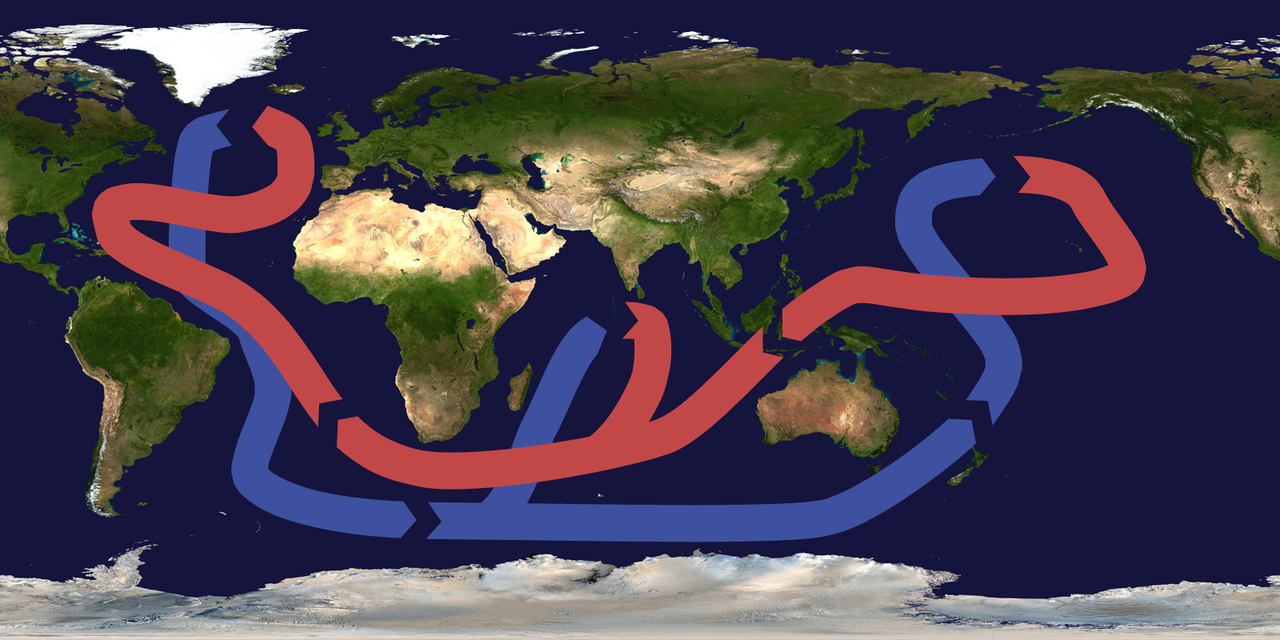
\includegraphics[width=\hsize]{chapters/4/1280px-Thermohaline_circulation.png}
\caption{
Das globale Förderband der thermohalinen Zirkulation.
\label{skript:thc:foerderband}}
\end{figure}%
Der Salzgehalt des Meerwassers ist nicht konstant,
hat aber ähnlich grossen Einfluss auf die Dichte wie die Temperatur.
Dies führt zu einer grossräumigen Zirkulationsströmung in den Weltmeeren,
genannt die thermohaline Zirkulation,
und damit zu einem weiteren bedeutenden Energietransportmechanismus.
Abbildung~\ref{skript:thc:foerderband} zeigt den Umfang der Zirkulation,
auch genannt das globale Förderband (conveyor belt).
Auf einer Zeitskala von Jahrzehnten bis Jahrhunderten wird Meerwasser 
und damit auch Wärmeenergie über Distanzen umgewälzt, welche mehrfach die
Erde umspannen.

Die Organismen, die in den oberen Wasserschichten absterben, sinken langsam
auf den Meeresgrund.
Ohne eine umfassende Umwälzung der Weltmeere würden die oberen Wasserschichten
mit der Zeit an Nährstoffen verarmen.
Die thermohaline Zirkulation stellt also auch die Versorgung der
Weltmeere mit Nährstoffen sicher.

Der Golfstrom ist ein kleiner Ausschnitt des globalen Förderbandes.
Die gut bekannte Bedeutung des Golfstroms für das europäische Klima 
deutet an, wie wichtig die thermohaline Zirkulation für das globale
Klima ist.
Es ist daher unerlässlich zu verstehen, was die Zirkulation antreibt und
wie sich der Klimawandel darauf auswirken könnte.

In diesem Kapitel soll die thermohaline Zirkulation modelliert werden.
Besonderes Augenmerk liegt dabei auf der Tatsache, dass dieses System
kippen kann.
Bei einer genügend grossen Änderung der Klimaparameter kann die Zirkulation
sich auf irreversible Art ändern.
Ein solches Ereignis hätte katastrophale Auswirkungen für das Klima.

\input{chapters/4/salinitaet.tex}
\input{chapters/4/schichtung.tex}
\input{chapters/4/box.tex}
\input{chapters/4/dimensionslos.tex}




%
% zonen.tex -- Zonenmodelle für das Klima
%
% (c) 2018 Prof Dr Andreas Müller, Hochschule Rapperswil
%
\chapter{Zonenmodelle\label{chapter:zonenmodelle}}
\lhead{Kapitel \thechapter: Zonenmodelle}
Die Erdrotation ist schnell im Vergleich zu den für typische Klimamodelle
wesentlichen Zeitspannen.
Wesentliche Aspekte der Klimaentwicklung sollten sich daher immer
noch modellieren lassen, wenn man den Zustand des Klimasystems über
die Erdrotation mittelt.
In diesem Kapitel werden daher vereinfachte Modelle diskutiert,
die nur die geographischen Länge als geometrischen Parameter haben.

\input{chapters/5/strahlung.tex}
\input{chapters/5/bilanz.tex}
\input{chapters/5/zonen.tex}
\input{chapters/5/spektral.tex}


%
% elnino.tex
%
% (c) 2018 Prof Dr Andreas Müller, Hochschule Rapperswil
%
\chapter{El Niño Southern Oscillation}
\lhead{El Niño Southern Oscillation}
Die Klimaentwicklung hängt wesentlich davon ab, wie Energie an der
Erdoberfläche verteilt wird.
Aus diesem Grund haben wir in Kapitel~\ref{chapter:fluiddynamik}
die Strömungsdynamik als den wesentlichen Mechanismus des 
Energietransportes in der Atmoshpäre studiert.
Und in Kapitel~\ref{chapter:thc} haben wir mit der Modellierung der
thermohalinen Zirkulation eine alternative Möglichkeit kennengelernt,
den Energie-Transport in den Weltmeeren zu beschreiben.

Das El Niño-Phänomen im Pazifik ist ein interessantes Teilsystem des
Klimasystems, welches einigermassen gut als isoliertes Teilsystem 
behandelt werden kann.
Die Modellierung, die wir in diesem Kapitel anstreben, braucht
einerseits die Ideen der Fluiddynamik, um die Energietransportmechanismen
zu beschreiben, und andererseits die Idee der Box-Modelle, um aus diesen
Mechanismen eine einfache gewöhnliche Differentiagleichung abzuleiten,
mit deren Hilfe die Dynamik des El~Niño studiert werden kann.

\section{El Niño}
\rhead{El Niño}

\input{chapters/7/kelvin.tex}
\input{chapters/7/rossby.tex}
\input{chapters/7/verzoegert.tex}


%
% assim.tex
%
% (c) 2018 Prof Dr Andreas Müller, Hochschule Rapperswil
%
\chapter{Datenassimilation}


\begin{appendices}
%\input{chapters/konstanten.tex}
%\input{chapters/komplexezahlen.tex}
\end{appendices}
\vfill
\pagebreak
\ifodd\value{page}\else\null\clearpage\fi
\lhead{Literatur}
\rhead{}
\printbibliography[heading=subbibliography]
\label{skript:literatur}
\end{refsection}

\part{Anwendungen und Weiterf"uhrende Themen}
\lhead{Anwendungen}
%
% uebersicht.tex -- Uebersicht ueber die Seminar-Arbeiten
%
% (c) 2018 Prof Dr Andreas Mueller, Hochschule Rapperswil
%
\chapter*{"Ubersicht}
\lhead{"Ubersicht}
\rhead{}
\label{skript:uebersicht}
Im zweiten Teil kommen die Teilnehmer des Seminars selbst zu Wort.
Die im ersten Teil dargelegten mathematischen Methoden und
grundlegenden Modelle werden dabei verfeinert, verallgemeinert
und auch numerisch überprüft.
Die Beispiele zeigen auch, dass umfassende Klimamodell erwartungsgemäss
schnell sehr komplex werden können.
Sie zeigen aber auch, dass es möglich ist, wesentliche Aspekte
des Klimas aus einfachen Überlegungen und mit übersichtlichen
mathematischen Modellen zu erfassen und zu verstehen.

{\em Matthias Baumann} und {\em Oliver Dias} zeigen zusätzliche
Informationen zum Lorenz-System, insbesondere zum Lorenz-Attraktor.
{\em Hansruedi Patzen} verallgemeinert das Vorgehen, mit dem das
Lorenz-System gewonnen wurde, im Sinne des Separationsverfahrens
für partielle Differentialgleichungen weiter, und gewinnt eine
Reihe von höherdimensionalen Lorenz-Systemen und untersucht weiter,
ob das beim dreidimensionalen System gefundene chaotische Verhalten 
auch in den höherdimensionalen Versionen zu finden ist.
Diese Untersuchungen zeigen, dass das Verhalten wahrscheinlich
nicht nur ein Artefakt der Reduktion auf drei Dimensionen ist, sondern
eine inhärente Eigenschaft des Lorenz-Systems.

Die exakte Lösung von Klimamodellen ist oft sehr schwierig, oft sind
Parameter oder Abhängigkeiten nicht bekannt.
Ein alternativer Ansatz ist daher, die zeitliche Entwicklung
im Sinne von machine learning zu lernen.
{\em Martin Stypinski} untersucht diesen Ansatz an zwei Beispielen,
der Wärmeleitungsgleichung und der nichtlinearen Gleichung von Burgers.
Die Beispiele zeigen vor allem auch, wie mathematisches Wissen über das
Modell hilft, die neuronalen Netzwerke zweckmässig zu entwerfen.

Die im Text entwickelten Modelle sind meist noch rudimentär, eine
reihe von Arbeiten haben sich daher mit Erweiterungen und Verfeinerungen
befasst.
{\em Jonas Gründler} hat das 2-Box Modell der thermohalinen Zirkulation
auf 3 Boxen verallgemeinert.
{\em Silvio Marti} studiert den Einfluss von Eis auf das Klima.
Die verzögerte Differentialgleichung des El Niño-Systems kann
numerische gelöst werden. {\em Raphael Unterer} zeigt, wie dies
funktioniert und findet insbesondere auch eine Stabilitätsbedingung
für sein Verfahren.
{\em Nicolas Tobler} hat versucht, die Modelle auf verschiedene
Planeten zu verallgemeinern und damit die Unterschiede der Atmosphären
der Planeten Venus, Erde und Mars zu erklären.
Die Einflüsse anderer Planeten zeigen sich zum Beispiel in der
Neigung der Erdachse gegen die Erdbahnebene.
Wie {\em Sebastian Lenhard} vorführt, können auch kleine Änderungen
der Neigung das Klima dramatisch verändern.
%Schliesslich gibt es auch eine Kopplung zwischen Klima und
%Vegetation, die {\em Matthias Dunkel} modelliert hat.

Die letzten zwei Kapitel befassen sich mit der Aufarbeitung der
Daten, auf grund derer wir zum Schluss kommen, dass 
der Klimawandel real ist.
Für Wetter- wie auch für Klimamodelle sind grosse Datenmengen
von Wetter- und Klimamessstationen in die Rechnung zu integrieren.
Der Kalman-Filter ist die Basis vieler moderner Lösungsansätze
für dieses Problem.
Am Beispiel des erweiterten Kalman-Filters für das Lorenz-System
zeigt {\em Michael Müller}, wie es möglich ist, den Systemzustand
selbst eines chaotischen nichtlinearen Systems zu 
Extreme Ereignisse sind in den letzten Jahren häufiger geworden
und werden oft als Indikatoren für die Klimaveränderung angeführt.
Wie man mit statistischen Daten über solche Ereignisse beweisen
kann, dass der Klimawandel tatsächlich stattfindet, zeigt
{\em Melina Staub}.






\def\chapterauthor#1{{\large #1}\bigskip\bigskip}
% Artikeverzoegert
%
% main.tex -- Paper zum Thema <thema>
%
% (c) 2018 Hochschule Rapperswil
%
\chapter{Achsneigung und Eiszeiten\label{chapter:thema}}
\lhead{Achseneigung und Eiszeiten}
\begin{refsection}
\chapterauthor{Sebastian Lenhard}

\section{Abschnitt}
\rhead{Abschnitt}

\section{Schlussfolgerung}
\rhead{Schlussfolgerung}

\printbibliography[heading=subbibliography]
\end{refsection}

%
% main.tex -- Paper zum Thema <thema>
%
% (c) 2018 Hochschule Rapperswil
%
\chapter{Achsneigung und Eiszeiten\label{chapter:thema}}
\lhead{Achseneigung und Eiszeiten}
\begin{refsection}
\chapterauthor{Sebastian Lenhard}

\section{Abschnitt}
\rhead{Abschnitt}

\section{Schlussfolgerung}
\rhead{Schlussfolgerung}

\printbibliography[heading=subbibliography]
\end{refsection}

%
% main.tex -- Paper zum Thema <thema>
%
% (c) 2018 Hochschule Rapperswil
%
\chapter{Achsneigung und Eiszeiten\label{chapter:thema}}
\lhead{Achseneigung und Eiszeiten}
\begin{refsection}
\chapterauthor{Sebastian Lenhard}

\section{Abschnitt}
\rhead{Abschnitt}

\section{Schlussfolgerung}
\rhead{Schlussfolgerung}

\printbibliography[heading=subbibliography]
\end{refsection}

%
% main.tex -- Paper zum Thema <thema>
%
% (c) 2018 Hochschule Rapperswil
%
\chapter{Achsneigung und Eiszeiten\label{chapter:thema}}
\lhead{Achseneigung und Eiszeiten}
\begin{refsection}
\chapterauthor{Sebastian Lenhard}

\section{Abschnitt}
\rhead{Abschnitt}

\section{Schlussfolgerung}
\rhead{Schlussfolgerung}

\printbibliography[heading=subbibliography]
\end{refsection}

%
% main.tex -- Paper zum Thema <thema>
%
% (c) 2018 Hochschule Rapperswil
%
\chapter{Achsneigung und Eiszeiten\label{chapter:thema}}
\lhead{Achseneigung und Eiszeiten}
\begin{refsection}
\chapterauthor{Sebastian Lenhard}

\section{Abschnitt}
\rhead{Abschnitt}

\section{Schlussfolgerung}
\rhead{Schlussfolgerung}

\printbibliography[heading=subbibliography]
\end{refsection}

%
% main.tex -- Paper zum Thema <thema>
%
% (c) 2018 Hochschule Rapperswil
%
\chapter{Achsneigung und Eiszeiten\label{chapter:thema}}
\lhead{Achseneigung und Eiszeiten}
\begin{refsection}
\chapterauthor{Sebastian Lenhard}

\section{Abschnitt}
\rhead{Abschnitt}

\section{Schlussfolgerung}
\rhead{Schlussfolgerung}

\printbibliography[heading=subbibliography]
\end{refsection}

%
% main.tex -- Paper zum Thema <thema>
%
% (c) 2018 Hochschule Rapperswil
%
\chapter{Achsneigung und Eiszeiten\label{chapter:thema}}
\lhead{Achseneigung und Eiszeiten}
\begin{refsection}
\chapterauthor{Sebastian Lenhard}

\section{Abschnitt}
\rhead{Abschnitt}

\section{Schlussfolgerung}
\rhead{Schlussfolgerung}

\printbibliography[heading=subbibliography]
\end{refsection}

%
% main.tex -- Paper zum Thema <thema>
%
% (c) 2018 Hochschule Rapperswil
%
\chapter{Achsneigung und Eiszeiten\label{chapter:thema}}
\lhead{Achseneigung und Eiszeiten}
\begin{refsection}
\chapterauthor{Sebastian Lenhard}

\section{Abschnitt}
\rhead{Abschnitt}

\section{Schlussfolgerung}
\rhead{Schlussfolgerung}

\printbibliography[heading=subbibliography]
\end{refsection}

%
% main.tex -- Paper zum Thema <thema>
%
% (c) 2018 Hochschule Rapperswil
%
\chapter{Achsneigung und Eiszeiten\label{chapter:thema}}
\lhead{Achseneigung und Eiszeiten}
\begin{refsection}
\chapterauthor{Sebastian Lenhard}

\section{Abschnitt}
\rhead{Abschnitt}

\section{Schlussfolgerung}
\rhead{Schlussfolgerung}

\printbibliography[heading=subbibliography]
\end{refsection}

%
% main.tex -- Paper zum Thema <thema>
%
% (c) 2018 Hochschule Rapperswil
%
\chapter{Achsneigung und Eiszeiten\label{chapter:thema}}
\lhead{Achseneigung und Eiszeiten}
\begin{refsection}
\chapterauthor{Sebastian Lenhard}

\section{Abschnitt}
\rhead{Abschnitt}

\section{Schlussfolgerung}
\rhead{Schlussfolgerung}

\printbibliography[heading=subbibliography]
\end{refsection}

%
% main.tex -- Paper zum Thema <thema>
%
% (c) 2018 Hochschule Rapperswil
%
\chapter{Achsneigung und Eiszeiten\label{chapter:thema}}
\lhead{Achseneigung und Eiszeiten}
\begin{refsection}
\chapterauthor{Sebastian Lenhard}

\section{Abschnitt}
\rhead{Abschnitt}

\section{Schlussfolgerung}
\rhead{Schlussfolgerung}

\printbibliography[heading=subbibliography]
\end{refsection}

\vfill
\pagebreak
\ifodd\value{page}\else\null\clearpage\fi
\lhead{Index}
\rhead{}
\addcontentsline{toc}{chapter}{\indexname}
%
% skript.tex -- Skript ueber Klimawandel
%
% (c) 2017 Prof. Dr. Andreas Mueller, HSR
%
\documentclass{book}
\usepackage{etex}
\usepackage{geometry}
\geometry{papersize={170mm,240mm},total={140mm,200mm},top=21mm,bindingoffset=10mm}
\usepackage[english,ngerman]{babel}
\usepackage[utf8]{inputenc}
\usepackage[T1]{fontenc}
\usepackage{cancel}
\usepackage{times}
\usepackage{amsmath,amscd}
\usepackage{amssymb}
\usepackage{amsfonts}
\usepackage{amsthm}
\usepackage{graphicx}
\usepackage{fancyhdr}
\usepackage{textcomp}
\usepackage{txfonts}
%\usepackage{alltt} 
\newcommand\hmmax{0}
\newcommand\bmmax{0}
\usepackage{bm}
\usepackage{verbatim}
\usepackage{paralist}
\usepackage{makeidx}
\usepackage{array}
%\usepackage[colorlinks=true]{hyperref}
\usepackage{hyperref}
\usepackage{tikz}
\usepackage{pgfplots}
\usepackage{pgfplotstable}
\usepackage{pdftexcmds}
\usepackage{pgfmath}
%\usepackage{placeins}
%\usepackage{subfigure}
\usepackage[autostyle=false,english=american]{csquotes}
%\usepackage{float}
%\usepackage{enumitem}
\usepackage{wasysym}
\usepackage{environ}
%\usepackage{pifont}
%\usepackage{feynmp}
\usepackage{appendix}
\usetikzlibrary{calc,intersections,through,backgrounds,graphs,positioning,shapes,arrows,fit}
\usetikzlibrary{patterns,decorations.pathreplacing}
\usetikzlibrary{decorations.pathreplacing}
\usetikzlibrary{external}
\usetikzlibrary{datavisualization}
\usepackage[europeanvoltages,
            europeancurrents,
            europeanresistors,   % rectangular shape
            americaninductors,   % "4-bumbs" shape
            europeanports,       % rectangular logic ports
            siunitx,             % #1<#2>
            emptydiodes,
            noarrowmos,
            smartlabels]         % lables are rotated in a smart way
           {circuitikz}          %
\usepackage{siunitx}
\usepackage{tabularx}
\usetikzlibrary{arrows}

\usepackage{algpseudocode}
\usepackage{algorithm}
\usepackage{gensymb}
\usepackage{mathtools}


% Matlab
\usepackage{listings}
\usepackage{color} %red, green, blue, yellow, cyan, magenta, black, white
\definecolor{mygreen}{RGB}{28,172,0} % color values Red, Green, Blue
\definecolor{mylilas}{RGB}{170,55,241}

\lstset{language=Matlab,%
    %basicstyle=\color{red},
    breaklines=true,%
    morekeywords={matlab2tikz},
    keywordstyle=\color{blue},%
    morekeywords=[2]{1}, keywordstyle=[2]{\color{black}},
    identifierstyle=\color{black},%
    stringstyle=\color{mylilas},
    commentstyle=\color{mygreen},%
    showstringspaces=false,%without this there will be a symbol in the places where there is a space
    numbers=left,%
    %numberstyle={\tiny \color{black}},% size of the numbers
    numbersep=9pt, % this defines how far the numbers are from the text
    emph=[1]{break},emphstyle=[1]\color{red}, %some words to emphasise
    %emph=[2]{word1,word2}, emphstyle=[2]{style},    
}
\lstdefinestyle{Matlab}{
  numbers=left,
  belowcaptionskip=1\baselineskip,
  breaklines=true,
  frame=L,
  xleftmargin=\parindent,
  language=Matlab,
  showstringspaces=false,
  basicstyle=\footnotesize\ttfamily,
  keywordstyle=\bfseries\color{green!40!black},
  commentstyle=\itshape\color{purple!40!black},
  identifierstyle=\color{blue},
  stringstyle=\color{orange},
  numberstyle=\ttfamily\tiny
}
\lstdefinelanguage{Matlab}{
  keywords={function,global,size,zeros,switch,case,otherwise,end,sin,cos,cot,floor,ode45,hold,polarplot},
  sensitive=true
}
\lstdefinelanguage{Maxima}{
  keywords={addrow,addcol,zeromatrix,ident,augcoefmatrix,ratsubst,sum,diff,ev,tex,%
    with_stdout,nouns,express,depends,load,length,submatrix,div,grad,curl,matrix,%
    invert,lambda,facsum,expand,false,then,if,else,subst,batchload,%
    rootscontract,solve,part,assume,sqrt,integrate,abs,inf,exp,sin,cos,sinh,cosh,taylor,ratsimp},
  sensitive=true,
  comment=[n][\itshape]{/*}{*/}
}
\lstdefinestyle{Maxima}{
  numbers=left,
  belowcaptionskip=1\baselineskip,
  breaklines=true,
  frame=L,
  xleftmargin=\parindent,
  language=Maxima,
  showstringspaces=false,
  basicstyle=\footnotesize\ttfamily,
  keywordstyle=\bfseries\color{green!40!black},
  commentstyle=\itshape\color{purple!40!black},
  identifierstyle=\color{blue},
  stringstyle=\color{orange},
  numberstyle=\ttfamily\tiny
}
\lstset{language=Octave,%
    %basicstyle=\color{red},
    breaklines=true,%
    morekeywords={function,global,size,zeros,switch,case,otherwise,end,sin,cos,cot,floor,ode45,hold,polarplot,endfunction,size,endswitch,cat,printf,for,endfor,if,return,endif,abs,while,endwhile},
    keywordstyle=\color{blue},%
    morekeywords=[2]{1}, keywordstyle=[2]{\color{black}},
    identifierstyle=\color{black},%
    stringstyle=\color{mylilas},
    commentstyle=\color{mygreen},%
    showstringspaces=false,%without this there will be a symbol in the places where there is a space
    numbers=left,%
    %numberstyle={\tiny \color{black}},% size of the numbers
    numbersep=9pt, % this defines how far the numbers are from the text
    emph=[1]{break},emphstyle=[1]\color{red}, %some words to emphasise
    %emph=[2]{word1,word2}, emphstyle=[2]{style},    
}
\lstdefinestyle{Octave}{
  numbers=left,
  belowcaptionskip=1\baselineskip,
  breaklines=true,
  frame=L,
  xleftmargin=\parindent,
  language=Octave,
  showstringspaces=false,
  basicstyle=\footnotesize\ttfamily,
  keywordstyle=\bfseries\color{green!40!black},
  commentstyle=\itshape\color{purple!40!black},
  identifierstyle=\color{blue},
  stringstyle=\color{orange},
  numberstyle=\ttfamily\tiny
}
\lstdefinestyle{C}{
  numbers=left,
  belowcaptionskip=1\baselineskip,
  breaklines=true,
  frame=L,
  xleftmargin=\parindent,
  language=C,
  showstringspaces=false,
  basicstyle=\footnotesize\ttfamily,
  keywordstyle=\bfseries\color{green!40!black},
  commentstyle=\itshape\color{purple!40!black},
  identifierstyle=\color{blue},
  stringstyle=\color{orange},
  numberstyle=\ttfamily\tiny
}
\usepackage{caption}
\usepackage[mode=buildnew]{standalone}
\usepackage[backend=bibtex]{biblatex}

% additional packages
%
% packages.tex -- zusätzliche Packages 
%
% In diesem File werden \usepackage{}-Aufrufe eingetragen für Packages, die
% noch nicht im skript.tex aufgerufen werden
%
% (c) 2018 Michael Müller, Hochschule Rapperswil
%


%
% packages.tex -- zusätzliche Packages 
%
% In diesem File werden \usepackage{}-Aufrufe eingetragen für Packages, die
% noch nicht im skript.tex aufgerufen werden
%
% (c) 2018 Michael Müller, Hochschule Rapperswil
%


%
% packages.tex -- zusätzliche Packages 
%
% In diesem File werden \usepackage{}-Aufrufe eingetragen für Packages, die
% noch nicht im skript.tex aufgerufen werden
%
% (c) 2018 Michael Müller, Hochschule Rapperswil
%


%
% packages.tex -- zusätzliche Packages 
%
% In diesem File werden \usepackage{}-Aufrufe eingetragen für Packages, die
% noch nicht im skript.tex aufgerufen werden
%
% (c) 2018 Michael Müller, Hochschule Rapperswil
%


%
% packages.tex -- zusätzliche Packages 
%
% In diesem File werden \usepackage{}-Aufrufe eingetragen für Packages, die
% noch nicht im skript.tex aufgerufen werden
%
% (c) 2018 Michael Müller, Hochschule Rapperswil
%


%
% packages.tex -- zusätzliche Packages 
%
% In diesem File werden \usepackage{}-Aufrufe eingetragen für Packages, die
% noch nicht im skript.tex aufgerufen werden
%
% (c) 2018 Michael Müller, Hochschule Rapperswil
%


%
% packages.tex -- zusätzliche Packages 
%
% In diesem File werden \usepackage{}-Aufrufe eingetragen für Packages, die
% noch nicht im skript.tex aufgerufen werden
%
% (c) 2018 Michael Müller, Hochschule Rapperswil
%


%
% packages.tex -- zusätzliche Packages 
%
% In diesem File werden \usepackage{}-Aufrufe eingetragen für Packages, die
% noch nicht im skript.tex aufgerufen werden
%
% (c) 2018 Michael Müller, Hochschule Rapperswil
%


%
% packages.tex -- zusätzliche Packages 
%
% In diesem File werden \usepackage{}-Aufrufe eingetragen für Packages, die
% noch nicht im skript.tex aufgerufen werden
%
% (c) 2018 Michael Müller, Hochschule Rapperswil
%


%
% packages.tex -- zusätzliche Packages 
%
% In diesem File werden \usepackage{}-Aufrufe eingetragen für Packages, die
% noch nicht im skript.tex aufgerufen werden
%
% (c) 2018 Michael Müller, Hochschule Rapperswil
%



% workaround for biblatex bug
\makeatletter
\def\blx@maxline{77}
\makeatother
\addbibresource{references.bib}
% Bibresources für jeden einzelnen Artikel
%\addbibresource{eis/references.bib}
%\addbibresource{extrem/references.bib}
%\addbibresource{kalman/references.bib}
%\addbibresource{learning/references.bib}
\addbibresource{lorenz/references.bib}
%\addbibresource{lorenz2/references.bib}
%\addbibresource{planeten/references.bib}
%\addbibresource{thermohalin/references.bib}
%\addbibresource{vegetation/references.bib}
%\addbibresource{verzoegert/references.bib}
\AtEndDocument{\clearpage\ifodd\value{page}\else\null\clearpage\fi}
\makeindex
%\pgfplotsset{compat=1.12}
\setlength{\headheight}{15pt} % fix headheight warning
\DeclareGraphicsRule{*}{mps}{*}{}
\begin{document}
\pagestyle{fancy}
\frontmatter
\newcommand\HRule{\noindent\rule{\linewidth}{1.5pt}}
\begin{titlepage}
\vspace*{\stretch{1}}
\HRule
\vspace*{5pt}
\begin{flushright}
{
\LARGE
Mathematisches Seminar\\
\vspace*{20pt}
\Huge
Klimawandel%
}
\vspace*{5pt}
\end{flushright}
\HRule
\begin{flushright}
\vspace{60pt}
\Large
Leitung: Andreas M"uller\\
\vspace{40pt}
\Large
%
% teilnehmer.tex -- Liste der Seminarteilnehmer für Titelseite
%
% (c) 2018 Prof Dr Andreas Müller, Hochschule Rapperswil
%
Matthias Baumann,
Oliver Dias-Lalcaca,
%Matthias Dunkel%,
Jonas Gründler%,
\\
Sebastian Lenhard,
Silvio Marti,
Michael~Müller,
Hansruedi~Patzen%,
\\
Melina~Staub,
Martin~Stypinski,
Nicolas Tobler,
Raphael Unterer
\\

%Matthias Baumann,
%Oliver Dias-Lalcaca,
%Matthias Dunkel%,
%\\
%Flurina Hoby,
%Sebastian Lenhard,
%Silvio Marti,
%Hansruedi~Patzen%,
%\\
%Melina~Staub,
%Martin~Stypinski,
%Nicolas Tobler,
%Raphael Unterer
\end{flushright}
\vspace*{\stretch{2}}
\begin{center}
Hochschule f"ur Technik, Rapperswil, 2018
\end{center}
\end{titlepage}
\hypersetup{
    linktoc=all,
    linkcolor=blue
}
\newcounter{beispiel}
\newenvironment{beispiele}{
\bgroup\smallskip\parindent0pt\bf Beispiele\egroup

\begin{list}{\arabic{beispiel}.}
  {\usecounter{beispiel}
  \setlength{\labelsep}{5mm}
  \setlength{\rightmargin}{0pt}
}}{\end{list}}
\newcounter{uebungsaufgabezaehler}
% environment fuer uebungsaufgaben
\newenvironment{uebungsaufgaben}{
\begin{list}{\arabic{uebungsaufgabezaehler}.}
  {\usecounter{uebungsaufgabezaehler}
  \setlength{\labelwidth}{2cm}
  \setlength{\leftmargin}{0pt}
  \setlength{\labelsep}{5mm}
  \setlength{\rightmargin}{0pt}
  \setlength{\itemindent}{0pt}
}}{\end{list}\vfill\pagebreak}
\newenvironment{teilaufgaben}{
\begin{enumerate}
\renewcommand{\labelenumi}{\alph{enumi})}
}{\end{enumerate}}
% Aufgabe
\newcounter{problemcounter}[chapter]
\def\aufgabenpath{chapters/uebungsaufgaben/}
\def\ainput#1{\input\aufgabenpath/#1}
\def\verbatimainput#1{\expandafter\verbatiminput{\aufgabenpath/#1}}
\def\aufgabetoplevel#1{%
\expandafter\def\expandafter\inputpath{#1}%
\let\aufgabepath=\inputpath
}
\def\includeagraphics[#1]#2{\expandafter\includegraphics[#1]{\aufgabepath#2}}
% \aufgabe
\newcommand{\uebungsaufgabe}[1]{%
\refstepcounter{problemcounter}%
\label{#1}%
\bigskip{\parindent0pt\strut}\hbox{\bf\arabic{problemcounter}. }%
\expandafter\def\csname aufgabenpath\endcsname{\inputpath/}%
\expandafter\input{chapters/uebungsaufgaben/#1.tex}
}
\renewcommand\theproblemcounter{\thechapter.\arabic{problemcounter}}

% Loesung
\def\swallow#1{
%nothing
}
\NewEnviron{loesung}[1][L"osung]{%
\begin{proof}[#1]%
\renewcommand{\qedsymbol}{$\bigcirc$}
\BODY
\end{proof}
}
\NewEnviron{bewertung}{%
\begin{proof}[Bewertung]%
\renewcommand{\qedsymbol}{}
\BODY
\end{proof}
}
\NewEnviron{diskussion}{%
\begin{proof}[Diskussion]%
\renewcommand{\qedsymbol}{}
\BODY
\end{proof}
}
\NewEnviron{hinweis}{%
\begin{proof}[Hinweis]%
\renewcommand{\qedsymbol}{}
\BODY
\end{proof}
}
\def\keineloesungen{%
\RenewEnviron{loesung}{\relax}
\RenewEnviron{bewertung}{\relax}
\RenewEnviron{diskussion}{\relax}
}
\newenvironment{beispiel}{%
\begin{proof}[Beispiel]%
\renewcommand{\qedsymbol}{$\bigcirc$}
}{\end{proof}}

\allowdisplaybreaks

\lhead{Inhaltsverzeichnis}
\rhead{}
\tableofcontents
\newtheorem{satz}{Satz}[chapter]
\newtheorem{hilfssatz}[satz]{Hilfssatz}
\newtheorem{definition}[satz]{Definition}
\newtheorem{annahme}[satz]{Annahme}
\newtheorem{problem}[satz]{Problem}
\newtheorem*{problem*}{Problem}
\renewcommand{\floatpagefraction}{0.7}
\mainmatter
%
% vorwort.tex -- Vorwort zum Buch zum Seminar
%
% (c) 2017 Prof Dr Andreas Mueller, Hochschule Rapperswil
%
\chapter*{Vorwort}
\lhead{Vorwort}
\rhead{}
Dieses Buch entstand im Rahmen des Mathematischen Seminars
im Frühjahrssemester 2017 an der Hochschule für Technik Rapperswil.
Die Teilnehmer, Studierende der Abteilungen für Elektrotechnik,
Informatik und Bauingenieurwesen der
HSR, erarbeiteten nach einer Einführung in das Themengebiet jeweils
einzelne Aspekte des Gebietes in Form einer Seminararbeit, über
deren Resultate sie auch in einem Vortrag informierten. 

Im Frühjahr 2018 war das Thema des Seminars der Klimawandel.

Im zweiten Teil dieses Skripts kommen dann die Teilnehmer selbst zu Wort.
Ihre Arbeiten wurden jeweils als einzelne
Kapitel mit meist nur typographischen Änderungen übernommen.
Diese weiterführenden Kapitel sind sehr verschiedenartig.
Eine Übersicht und Einführung findet sich in der Einleitung
zum zweiten Teil auf Seite~\pageref{skript:uebersicht}.

In einigen Arbeiten wurde auch Code zur Demonstration der 
besprochenen Methoden und Resultate geschrieben, soweit
möglich und sinnvoll wurde dieser Code im Github-Repository
dieses Kurses%
\footnote{\url{https://github.com/AndreasFMueller/SeminarKlima.git}}
abgelegt.

Im genannten Repository findet sich auch der Source-Code dieses
Skriptes, es wird hier unter einer Creative Commons Lizenz
zur Verfügung gestellt.
Auf der beiliegenden DVD befinden sich die Testdaten und Programme
zu zwei der simulationsintensiveren Artikel im zweiten Teil.



\part{Grundlagen}
%\keineloesungen
\begin{refsection}
%
% part1.tex
%
% (c) 2018 Prof Dr Andreas Müller, Hochschule Rapperswil
%
\input{chapters/wuk.tex}
\input{chapters/dgl.tex}
\input{chapters/thc.tex}
\input{chapters/zonen.tex}
\input{chapters/elnino.tex}
\input{chapters/assim.tex}

\begin{appendices}
%\input{chapters/konstanten.tex}
%\input{chapters/komplexezahlen.tex}
\end{appendices}
\vfill
\pagebreak
\ifodd\value{page}\else\null\clearpage\fi
\lhead{Literatur}
\rhead{}
\printbibliography[heading=subbibliography]
\label{skript:literatur}
\end{refsection}

\part{Anwendungen und Weiterf"uhrende Themen}
\lhead{Anwendungen}
%
% uebersicht.tex -- Uebersicht ueber die Seminar-Arbeiten
%
% (c) 2018 Prof Dr Andreas Mueller, Hochschule Rapperswil
%
\chapter*{"Ubersicht}
\lhead{"Ubersicht}
\rhead{}
\label{skript:uebersicht}
Im zweiten Teil kommen die Teilnehmer des Seminars selbst zu Wort.
Die im ersten Teil dargelegten mathematischen Methoden und
grundlegenden Modelle werden dabei verfeinert, verallgemeinert
und auch numerisch überprüft.
Die Beispiele zeigen auch, dass umfassende Klimamodell erwartungsgemäss
schnell sehr komplex werden können.
Sie zeigen aber auch, dass es möglich ist, wesentliche Aspekte
des Klimas aus einfachen Überlegungen und mit übersichtlichen
mathematischen Modellen zu erfassen und zu verstehen.

{\em Matthias Baumann} und {\em Oliver Dias} zeigen zusätzliche
Informationen zum Lorenz-System, insbesondere zum Lorenz-Attraktor.
{\em Hansruedi Patzen} verallgemeinert das Vorgehen, mit dem das
Lorenz-System gewonnen wurde, im Sinne des Separationsverfahrens
für partielle Differentialgleichungen weiter, und gewinnt eine
Reihe von höherdimensionalen Lorenz-Systemen und untersucht weiter,
ob das beim dreidimensionalen System gefundene chaotische Verhalten 
auch in den höherdimensionalen Versionen zu finden ist.
Diese Untersuchungen zeigen, dass das Verhalten wahrscheinlich
nicht nur ein Artefakt der Reduktion auf drei Dimensionen ist, sondern
eine inhärente Eigenschaft des Lorenz-Systems.

Die exakte Lösung von Klimamodellen ist oft sehr schwierig, oft sind
Parameter oder Abhängigkeiten nicht bekannt.
Ein alternativer Ansatz ist daher, die zeitliche Entwicklung
im Sinne von machine learning zu lernen.
{\em Martin Stypinski} untersucht diesen Ansatz an zwei Beispielen,
der Wärmeleitungsgleichung und der nichtlinearen Gleichung von Burgers.
Die Beispiele zeigen vor allem auch, wie mathematisches Wissen über das
Modell hilft, die neuronalen Netzwerke zweckmässig zu entwerfen.

Die im Text entwickelten Modelle sind meist noch rudimentär, eine
reihe von Arbeiten haben sich daher mit Erweiterungen und Verfeinerungen
befasst.
{\em Jonas Gründler} hat das 2-Box Modell der thermohalinen Zirkulation
auf 3 Boxen verallgemeinert.
{\em Silvio Marti} studiert den Einfluss von Eis auf das Klima.
Die verzögerte Differentialgleichung des El Niño-Systems kann
numerische gelöst werden. {\em Raphael Unterer} zeigt, wie dies
funktioniert und findet insbesondere auch eine Stabilitätsbedingung
für sein Verfahren.
{\em Nicolas Tobler} hat versucht, die Modelle auf verschiedene
Planeten zu verallgemeinern und damit die Unterschiede der Atmosphären
der Planeten Venus, Erde und Mars zu erklären.
Die Einflüsse anderer Planeten zeigen sich zum Beispiel in der
Neigung der Erdachse gegen die Erdbahnebene.
Wie {\em Sebastian Lenhard} vorführt, können auch kleine Änderungen
der Neigung das Klima dramatisch verändern.
%Schliesslich gibt es auch eine Kopplung zwischen Klima und
%Vegetation, die {\em Matthias Dunkel} modelliert hat.

Die letzten zwei Kapitel befassen sich mit der Aufarbeitung der
Daten, auf grund derer wir zum Schluss kommen, dass 
der Klimawandel real ist.
Für Wetter- wie auch für Klimamodelle sind grosse Datenmengen
von Wetter- und Klimamessstationen in die Rechnung zu integrieren.
Der Kalman-Filter ist die Basis vieler moderner Lösungsansätze
für dieses Problem.
Am Beispiel des erweiterten Kalman-Filters für das Lorenz-System
zeigt {\em Michael Müller}, wie es möglich ist, den Systemzustand
selbst eines chaotischen nichtlinearen Systems zu 
Extreme Ereignisse sind in den letzten Jahren häufiger geworden
und werden oft als Indikatoren für die Klimaveränderung angeführt.
Wie man mit statistischen Daten über solche Ereignisse beweisen
kann, dass der Klimawandel tatsächlich stattfindet, zeigt
{\em Melina Staub}.






\def\chapterauthor#1{{\large #1}\bigskip\bigskip}
% Artikeverzoegert
%
% main.tex -- Paper zum Thema <thema>
%
% (c) 2018 Hochschule Rapperswil
%
\chapter{Achsneigung und Eiszeiten\label{chapter:thema}}
\lhead{Achseneigung und Eiszeiten}
\begin{refsection}
\chapterauthor{Sebastian Lenhard}

\section{Abschnitt}
\rhead{Abschnitt}

\section{Schlussfolgerung}
\rhead{Schlussfolgerung}

\printbibliography[heading=subbibliography]
\end{refsection}

%
% main.tex -- Paper zum Thema <thema>
%
% (c) 2018 Hochschule Rapperswil
%
\chapter{Achsneigung und Eiszeiten\label{chapter:thema}}
\lhead{Achseneigung und Eiszeiten}
\begin{refsection}
\chapterauthor{Sebastian Lenhard}

\section{Abschnitt}
\rhead{Abschnitt}

\section{Schlussfolgerung}
\rhead{Schlussfolgerung}

\printbibliography[heading=subbibliography]
\end{refsection}

%
% main.tex -- Paper zum Thema <thema>
%
% (c) 2018 Hochschule Rapperswil
%
\chapter{Achsneigung und Eiszeiten\label{chapter:thema}}
\lhead{Achseneigung und Eiszeiten}
\begin{refsection}
\chapterauthor{Sebastian Lenhard}

\section{Abschnitt}
\rhead{Abschnitt}

\section{Schlussfolgerung}
\rhead{Schlussfolgerung}

\printbibliography[heading=subbibliography]
\end{refsection}

%
% main.tex -- Paper zum Thema <thema>
%
% (c) 2018 Hochschule Rapperswil
%
\chapter{Achsneigung und Eiszeiten\label{chapter:thema}}
\lhead{Achseneigung und Eiszeiten}
\begin{refsection}
\chapterauthor{Sebastian Lenhard}

\section{Abschnitt}
\rhead{Abschnitt}

\section{Schlussfolgerung}
\rhead{Schlussfolgerung}

\printbibliography[heading=subbibliography]
\end{refsection}

%
% main.tex -- Paper zum Thema <thema>
%
% (c) 2018 Hochschule Rapperswil
%
\chapter{Achsneigung und Eiszeiten\label{chapter:thema}}
\lhead{Achseneigung und Eiszeiten}
\begin{refsection}
\chapterauthor{Sebastian Lenhard}

\section{Abschnitt}
\rhead{Abschnitt}

\section{Schlussfolgerung}
\rhead{Schlussfolgerung}

\printbibliography[heading=subbibliography]
\end{refsection}

%
% main.tex -- Paper zum Thema <thema>
%
% (c) 2018 Hochschule Rapperswil
%
\chapter{Achsneigung und Eiszeiten\label{chapter:thema}}
\lhead{Achseneigung und Eiszeiten}
\begin{refsection}
\chapterauthor{Sebastian Lenhard}

\section{Abschnitt}
\rhead{Abschnitt}

\section{Schlussfolgerung}
\rhead{Schlussfolgerung}

\printbibliography[heading=subbibliography]
\end{refsection}

%
% main.tex -- Paper zum Thema <thema>
%
% (c) 2018 Hochschule Rapperswil
%
\chapter{Achsneigung und Eiszeiten\label{chapter:thema}}
\lhead{Achseneigung und Eiszeiten}
\begin{refsection}
\chapterauthor{Sebastian Lenhard}

\section{Abschnitt}
\rhead{Abschnitt}

\section{Schlussfolgerung}
\rhead{Schlussfolgerung}

\printbibliography[heading=subbibliography]
\end{refsection}

%
% main.tex -- Paper zum Thema <thema>
%
% (c) 2018 Hochschule Rapperswil
%
\chapter{Achsneigung und Eiszeiten\label{chapter:thema}}
\lhead{Achseneigung und Eiszeiten}
\begin{refsection}
\chapterauthor{Sebastian Lenhard}

\section{Abschnitt}
\rhead{Abschnitt}

\section{Schlussfolgerung}
\rhead{Schlussfolgerung}

\printbibliography[heading=subbibliography]
\end{refsection}

%
% main.tex -- Paper zum Thema <thema>
%
% (c) 2018 Hochschule Rapperswil
%
\chapter{Achsneigung und Eiszeiten\label{chapter:thema}}
\lhead{Achseneigung und Eiszeiten}
\begin{refsection}
\chapterauthor{Sebastian Lenhard}

\section{Abschnitt}
\rhead{Abschnitt}

\section{Schlussfolgerung}
\rhead{Schlussfolgerung}

\printbibliography[heading=subbibliography]
\end{refsection}

%
% main.tex -- Paper zum Thema <thema>
%
% (c) 2018 Hochschule Rapperswil
%
\chapter{Achsneigung und Eiszeiten\label{chapter:thema}}
\lhead{Achseneigung und Eiszeiten}
\begin{refsection}
\chapterauthor{Sebastian Lenhard}

\section{Abschnitt}
\rhead{Abschnitt}

\section{Schlussfolgerung}
\rhead{Schlussfolgerung}

\printbibliography[heading=subbibliography]
\end{refsection}

%
% main.tex -- Paper zum Thema <thema>
%
% (c) 2018 Hochschule Rapperswil
%
\chapter{Achsneigung und Eiszeiten\label{chapter:thema}}
\lhead{Achseneigung und Eiszeiten}
\begin{refsection}
\chapterauthor{Sebastian Lenhard}

\section{Abschnitt}
\rhead{Abschnitt}

\section{Schlussfolgerung}
\rhead{Schlussfolgerung}

\printbibliography[heading=subbibliography]
\end{refsection}

\vfill
\pagebreak
\ifodd\value{page}\else\null\clearpage\fi
\lhead{Index}
\rhead{}
\addcontentsline{toc}{chapter}{\indexname}
%
% skript.tex -- Skript ueber Klimawandel
%
% (c) 2017 Prof. Dr. Andreas Mueller, HSR
%
\documentclass{book}
\usepackage{etex}
\usepackage{geometry}
\geometry{papersize={170mm,240mm},total={140mm,200mm},top=21mm,bindingoffset=10mm}
\usepackage[english,ngerman]{babel}
\usepackage[utf8]{inputenc}
\usepackage[T1]{fontenc}
\usepackage{cancel}
\usepackage{times}
\usepackage{amsmath,amscd}
\usepackage{amssymb}
\usepackage{amsfonts}
\usepackage{amsthm}
\usepackage{graphicx}
\usepackage{fancyhdr}
\usepackage{textcomp}
\usepackage{txfonts}
%\usepackage{alltt} 
\newcommand\hmmax{0}
\newcommand\bmmax{0}
\usepackage{bm}
\usepackage{verbatim}
\usepackage{paralist}
\usepackage{makeidx}
\usepackage{array}
%\usepackage[colorlinks=true]{hyperref}
\usepackage{hyperref}
\usepackage{tikz}
\usepackage{pgfplots}
\usepackage{pgfplotstable}
\usepackage{pdftexcmds}
\usepackage{pgfmath}
%\usepackage{placeins}
%\usepackage{subfigure}
\usepackage[autostyle=false,english=american]{csquotes}
%\usepackage{float}
%\usepackage{enumitem}
\usepackage{wasysym}
\usepackage{environ}
%\usepackage{pifont}
%\usepackage{feynmp}
\usepackage{appendix}
\usetikzlibrary{calc,intersections,through,backgrounds,graphs,positioning,shapes,arrows,fit}
\usetikzlibrary{patterns,decorations.pathreplacing}
\usetikzlibrary{decorations.pathreplacing}
\usetikzlibrary{external}
\usetikzlibrary{datavisualization}
\usepackage[europeanvoltages,
            europeancurrents,
            europeanresistors,   % rectangular shape
            americaninductors,   % "4-bumbs" shape
            europeanports,       % rectangular logic ports
            siunitx,             % #1<#2>
            emptydiodes,
            noarrowmos,
            smartlabels]         % lables are rotated in a smart way
           {circuitikz}          %
\usepackage{siunitx}
\usepackage{tabularx}
\usetikzlibrary{arrows}

\usepackage{algpseudocode}
\usepackage{algorithm}
\usepackage{gensymb}
\usepackage{mathtools}


% Matlab
\usepackage{listings}
\usepackage{color} %red, green, blue, yellow, cyan, magenta, black, white
\definecolor{mygreen}{RGB}{28,172,0} % color values Red, Green, Blue
\definecolor{mylilas}{RGB}{170,55,241}

\lstset{language=Matlab,%
    %basicstyle=\color{red},
    breaklines=true,%
    morekeywords={matlab2tikz},
    keywordstyle=\color{blue},%
    morekeywords=[2]{1}, keywordstyle=[2]{\color{black}},
    identifierstyle=\color{black},%
    stringstyle=\color{mylilas},
    commentstyle=\color{mygreen},%
    showstringspaces=false,%without this there will be a symbol in the places where there is a space
    numbers=left,%
    %numberstyle={\tiny \color{black}},% size of the numbers
    numbersep=9pt, % this defines how far the numbers are from the text
    emph=[1]{break},emphstyle=[1]\color{red}, %some words to emphasise
    %emph=[2]{word1,word2}, emphstyle=[2]{style},    
}
\lstdefinestyle{Matlab}{
  numbers=left,
  belowcaptionskip=1\baselineskip,
  breaklines=true,
  frame=L,
  xleftmargin=\parindent,
  language=Matlab,
  showstringspaces=false,
  basicstyle=\footnotesize\ttfamily,
  keywordstyle=\bfseries\color{green!40!black},
  commentstyle=\itshape\color{purple!40!black},
  identifierstyle=\color{blue},
  stringstyle=\color{orange},
  numberstyle=\ttfamily\tiny
}
\lstdefinelanguage{Matlab}{
  keywords={function,global,size,zeros,switch,case,otherwise,end,sin,cos,cot,floor,ode45,hold,polarplot},
  sensitive=true
}
\lstdefinelanguage{Maxima}{
  keywords={addrow,addcol,zeromatrix,ident,augcoefmatrix,ratsubst,sum,diff,ev,tex,%
    with_stdout,nouns,express,depends,load,length,submatrix,div,grad,curl,matrix,%
    invert,lambda,facsum,expand,false,then,if,else,subst,batchload,%
    rootscontract,solve,part,assume,sqrt,integrate,abs,inf,exp,sin,cos,sinh,cosh,taylor,ratsimp},
  sensitive=true,
  comment=[n][\itshape]{/*}{*/}
}
\lstdefinestyle{Maxima}{
  numbers=left,
  belowcaptionskip=1\baselineskip,
  breaklines=true,
  frame=L,
  xleftmargin=\parindent,
  language=Maxima,
  showstringspaces=false,
  basicstyle=\footnotesize\ttfamily,
  keywordstyle=\bfseries\color{green!40!black},
  commentstyle=\itshape\color{purple!40!black},
  identifierstyle=\color{blue},
  stringstyle=\color{orange},
  numberstyle=\ttfamily\tiny
}
\lstset{language=Octave,%
    %basicstyle=\color{red},
    breaklines=true,%
    morekeywords={function,global,size,zeros,switch,case,otherwise,end,sin,cos,cot,floor,ode45,hold,polarplot,endfunction,size,endswitch,cat,printf,for,endfor,if,return,endif,abs,while,endwhile},
    keywordstyle=\color{blue},%
    morekeywords=[2]{1}, keywordstyle=[2]{\color{black}},
    identifierstyle=\color{black},%
    stringstyle=\color{mylilas},
    commentstyle=\color{mygreen},%
    showstringspaces=false,%without this there will be a symbol in the places where there is a space
    numbers=left,%
    %numberstyle={\tiny \color{black}},% size of the numbers
    numbersep=9pt, % this defines how far the numbers are from the text
    emph=[1]{break},emphstyle=[1]\color{red}, %some words to emphasise
    %emph=[2]{word1,word2}, emphstyle=[2]{style},    
}
\lstdefinestyle{Octave}{
  numbers=left,
  belowcaptionskip=1\baselineskip,
  breaklines=true,
  frame=L,
  xleftmargin=\parindent,
  language=Octave,
  showstringspaces=false,
  basicstyle=\footnotesize\ttfamily,
  keywordstyle=\bfseries\color{green!40!black},
  commentstyle=\itshape\color{purple!40!black},
  identifierstyle=\color{blue},
  stringstyle=\color{orange},
  numberstyle=\ttfamily\tiny
}
\lstdefinestyle{C}{
  numbers=left,
  belowcaptionskip=1\baselineskip,
  breaklines=true,
  frame=L,
  xleftmargin=\parindent,
  language=C,
  showstringspaces=false,
  basicstyle=\footnotesize\ttfamily,
  keywordstyle=\bfseries\color{green!40!black},
  commentstyle=\itshape\color{purple!40!black},
  identifierstyle=\color{blue},
  stringstyle=\color{orange},
  numberstyle=\ttfamily\tiny
}
\usepackage{caption}
\usepackage[mode=buildnew]{standalone}
\usepackage[backend=bibtex]{biblatex}

% additional packages
\input{eis/packages.tex}
\input{extrem/packages.tex}
\input{kalman/packages.tex}
\input{learning/packages.tex}
\input{lorenz/packages.tex}
\input{lorenz2/packages.tex}
\input{planeten/packages.tex}
\input{thermohalin/packages.tex}
\input{vegetation/packages.tex}
\input{verzoegert/packages.tex}

% workaround for biblatex bug
\makeatletter
\def\blx@maxline{77}
\makeatother
\addbibresource{references.bib}
% Bibresources für jeden einzelnen Artikel
%\addbibresource{eis/references.bib}
%\addbibresource{extrem/references.bib}
%\addbibresource{kalman/references.bib}
%\addbibresource{learning/references.bib}
\addbibresource{lorenz/references.bib}
%\addbibresource{lorenz2/references.bib}
%\addbibresource{planeten/references.bib}
%\addbibresource{thermohalin/references.bib}
%\addbibresource{vegetation/references.bib}
%\addbibresource{verzoegert/references.bib}
\AtEndDocument{\clearpage\ifodd\value{page}\else\null\clearpage\fi}
\makeindex
%\pgfplotsset{compat=1.12}
\setlength{\headheight}{15pt} % fix headheight warning
\DeclareGraphicsRule{*}{mps}{*}{}
\begin{document}
\pagestyle{fancy}
\frontmatter
\newcommand\HRule{\noindent\rule{\linewidth}{1.5pt}}
\begin{titlepage}
\vspace*{\stretch{1}}
\HRule
\vspace*{5pt}
\begin{flushright}
{
\LARGE
Mathematisches Seminar\\
\vspace*{20pt}
\Huge
Klimawandel%
}
\vspace*{5pt}
\end{flushright}
\HRule
\begin{flushright}
\vspace{60pt}
\Large
Leitung: Andreas M"uller\\
\vspace{40pt}
\Large
\input{teilnehmer.tex}
%Matthias Baumann,
%Oliver Dias-Lalcaca,
%Matthias Dunkel%,
%\\
%Flurina Hoby,
%Sebastian Lenhard,
%Silvio Marti,
%Hansruedi~Patzen%,
%\\
%Melina~Staub,
%Martin~Stypinski,
%Nicolas Tobler,
%Raphael Unterer
\end{flushright}
\vspace*{\stretch{2}}
\begin{center}
Hochschule f"ur Technik, Rapperswil, 2018
\end{center}
\end{titlepage}
\hypersetup{
    linktoc=all,
    linkcolor=blue
}
\newcounter{beispiel}
\newenvironment{beispiele}{
\bgroup\smallskip\parindent0pt\bf Beispiele\egroup

\begin{list}{\arabic{beispiel}.}
  {\usecounter{beispiel}
  \setlength{\labelsep}{5mm}
  \setlength{\rightmargin}{0pt}
}}{\end{list}}
\newcounter{uebungsaufgabezaehler}
% environment fuer uebungsaufgaben
\newenvironment{uebungsaufgaben}{
\begin{list}{\arabic{uebungsaufgabezaehler}.}
  {\usecounter{uebungsaufgabezaehler}
  \setlength{\labelwidth}{2cm}
  \setlength{\leftmargin}{0pt}
  \setlength{\labelsep}{5mm}
  \setlength{\rightmargin}{0pt}
  \setlength{\itemindent}{0pt}
}}{\end{list}\vfill\pagebreak}
\newenvironment{teilaufgaben}{
\begin{enumerate}
\renewcommand{\labelenumi}{\alph{enumi})}
}{\end{enumerate}}
% Aufgabe
\newcounter{problemcounter}[chapter]
\def\aufgabenpath{chapters/uebungsaufgaben/}
\def\ainput#1{\input\aufgabenpath/#1}
\def\verbatimainput#1{\expandafter\verbatiminput{\aufgabenpath/#1}}
\def\aufgabetoplevel#1{%
\expandafter\def\expandafter\inputpath{#1}%
\let\aufgabepath=\inputpath
}
\def\includeagraphics[#1]#2{\expandafter\includegraphics[#1]{\aufgabepath#2}}
% \aufgabe
\newcommand{\uebungsaufgabe}[1]{%
\refstepcounter{problemcounter}%
\label{#1}%
\bigskip{\parindent0pt\strut}\hbox{\bf\arabic{problemcounter}. }%
\expandafter\def\csname aufgabenpath\endcsname{\inputpath/}%
\expandafter\input{chapters/uebungsaufgaben/#1.tex}
}
\renewcommand\theproblemcounter{\thechapter.\arabic{problemcounter}}

% Loesung
\def\swallow#1{
%nothing
}
\NewEnviron{loesung}[1][L"osung]{%
\begin{proof}[#1]%
\renewcommand{\qedsymbol}{$\bigcirc$}
\BODY
\end{proof}
}
\NewEnviron{bewertung}{%
\begin{proof}[Bewertung]%
\renewcommand{\qedsymbol}{}
\BODY
\end{proof}
}
\NewEnviron{diskussion}{%
\begin{proof}[Diskussion]%
\renewcommand{\qedsymbol}{}
\BODY
\end{proof}
}
\NewEnviron{hinweis}{%
\begin{proof}[Hinweis]%
\renewcommand{\qedsymbol}{}
\BODY
\end{proof}
}
\def\keineloesungen{%
\RenewEnviron{loesung}{\relax}
\RenewEnviron{bewertung}{\relax}
\RenewEnviron{diskussion}{\relax}
}
\newenvironment{beispiel}{%
\begin{proof}[Beispiel]%
\renewcommand{\qedsymbol}{$\bigcirc$}
}{\end{proof}}

\allowdisplaybreaks

\lhead{Inhaltsverzeichnis}
\rhead{}
\tableofcontents
\newtheorem{satz}{Satz}[chapter]
\newtheorem{hilfssatz}[satz]{Hilfssatz}
\newtheorem{definition}[satz]{Definition}
\newtheorem{annahme}[satz]{Annahme}
\newtheorem{problem}[satz]{Problem}
\newtheorem*{problem*}{Problem}
\renewcommand{\floatpagefraction}{0.7}
\mainmatter
\input{vorwort.tex}
\part{Grundlagen}
%\keineloesungen
\begin{refsection}
\input{chapters/part1.tex}
\begin{appendices}
%\input{chapters/konstanten.tex}
%\input{chapters/komplexezahlen.tex}
\end{appendices}
\vfill
\pagebreak
\ifodd\value{page}\else\null\clearpage\fi
\lhead{Literatur}
\rhead{}
\printbibliography[heading=subbibliography]
\label{skript:literatur}
\end{refsection}

\part{Anwendungen und Weiterf"uhrende Themen}
\lhead{Anwendungen}
\input{uebersicht.tex}
\def\chapterauthor#1{{\large #1}\bigskip\bigskip}
% Artikeverzoegert
\input{eis/main.tex}
\input{extrem/main.tex}
\input{kalman/main.tex}
\input{learning/main.tex}
\input{lorenz/main.tex}
\input{lorenz2/main.tex}
\input{neigung/main.tex}
\input{planeten/main.tex}
\input{thermohalin/main.tex}
\input{vegetation/main.tex}
\input{verzoegert/main.tex}
\vfill
\pagebreak
\ifodd\value{page}\else\null\clearpage\fi
\lhead{Index}
\rhead{}
\addcontentsline{toc}{chapter}{\indexname}
\input{skript.ind}

\end{document}


\end{document}


\end{document}


\end{document}
